\documentclass[bsc,letterpaper,12pt]{csthesis}
%\documentclass[letterpaper,12pt,twoside]{csthesis} % para imprimir de lado y lado


\paperwidth = 21.6cm		% Tamaño de la hoja
\paperheight = 27.9cm

%Margenes horizontales
\hoffset = -2.54cm		% Se elimna el offset horizontal
\oddsidemargin = 4cm
\evensidemargin = 2cm
\textwidth = 15.6cm

%Margenes verticales
\voffset = -2.54cm
\topmargin = 3cm
\headheight = 0cm
\headsep = 0cm
\textheight = 21.9cm
\footskip = 1cm


\usepackage[spanish,USenglish]{babel}     % Idioma Capitulos y demas
\usepackage[utf8]{inputenc}
\usepackage{lmodern}
\usepackage[T1]{fontenc}
\usepackage{cc/CreativeCommons}  %Licencia

\usepackage{listings} % Ingresar Codigo Fuente
\usepackage{verbatim}
\usepackage{moreverb}
\let\verbatiminput=\verbatimtabinput
\def\verbatimtabsize{8}  % Tabulación en verbatim

% Paquete para el manejo de hipervinculos
\usepackage[b5paper, breaklinks=true, pdfborder={0 0 0},colorlinks=false,pageanchor=true, 
plainpages=false,bookmarksopen=true,bookmarksopenlevel=3, hyperfootnotes=false]{hyperref}

% Paquete para el manejo de tablas
\usepackage{supertabular}

% Paquetes para simbolos
%\usepackage{mathcomp}
\usepackage{latexsym}
\usepackage{pifont}
\usepackage{amsfonts}
\usepackage{amssymb}
\usepackage{wasysym}
\usepackage{colortbl}
\usepackage{multicol} 
\usepackage{booktabs}
\usepackage{multirow}
\usepackage{algorithmic}
\usepackage[Algoritmo]{algorithm}
\usepackage{subfigure}


% Manejo de imagenes PDF y EPS
\newif\ifpdf
\ifx\pdfoutput\undefined
\pdffalse % we are not running PDFLaTeX
\else
\pdfoutput=1 % we are running PDFLaTeX
\pdftrue
\fi

\ifpdf
\usepackage[pdftex]{graphicx}
\else
\usepackage{graphicx}
\fi

\ifpdf
\DeclareGraphicsExtensions{.pdf, .jpg, .tif}
\else
\DeclareGraphicsExtensions{.eps, .jpg}
\fi

% Sangria de comienzo de parrafo
\setlength{\parindent}{0cm}
% Espacio vertical entre dos parrfos
\setlength{\parskip}{0.3cm}

% Definir el nombre de listas
\addto\captionsspanish{%
  \def\prefacename{Prefacio}%
  \def\refname{REFERENCIAS}%
  \def\abstractname{RESUMEN}%
  \def\bibname{REFERENCIAS}%
  \def\chaptername{Cap\'{\i}tulo}%
  \def\appendixname{Anexo}%
  \def\listfigurename{Lista de figuras}%
  \def\listtablename{Lista de cuadros}%
  \def\indexname{\'Indice alfab\'etico}%
  \def\figurename{Figura}%
  \def\tablename{Tabla}%
  \def\partname{Parte}%
  \def\enclname{Adjunto}%
  \def\ccname{Copia a}%
  \def\headtoname{A}%
  \def\pagename{P\'agina}%
  \def\seename{v\'ease}%
  \def\alsoname{v\'ease tambi\'en}%
  \def\proofname{Demostraci\'on}%
  \def\glossaryname{Glosario}}
  \addto\captionsspanish{\def\contentsname{CONTENIDO}}
  
\addto\captionsUSenglish{
  \def\abstractname{ABSTRACT}%
}  

%para rotar tablas  
\usepackage{rotating}



%partir palabras
\hyphenation{di-fe-ren-cia pro-pues-to pro-ble-mas po-pu-la-res cons-truccio-nes ne-ce-sa-ria-men-te}

% Inico del documento
\begin{document}
\selectlanguage{spanish}
\pagestyle{empty}% Sin número de página
%%% PORTADA


\thispagestyle{empty}
\vspace*{1 mm}
\begin{center}{\centering \large Aplicación de técnicas de minería de texto  para el descubrimiento de relaciones conceptuales
entre los trabajos de grado de la Universidad de Nariño}
\end{center}

\vspace{2.5cm}

\begin{center}{\large Jimmy Mateo Guerrero Restrepo}
\end{center}

\vspace{1.5cm}

\begin{figure}[!h]
\begin{center}

\includegraphics[scale=0.7]{pictures/uba.png}%logo of your university
\end{center}
\end{figure}

\vspace{3.5cm}

\begin{center}{\large Universidad de Buenos Aires\\
Facultad de Ciencias Exactas y Naturales\\
Departamento de Computación\\
Maestría Explotación de Datos y Descubrimiento del Conocimiento\\
Buenos Aires Argentina\\
2020}
\end{center}



\pagebreak

\newpage

% CONTRAPORTADA

\thispagestyle{empty}

\vspace*{1 mm}
\begin{center}{\centering \large Aplicación de técnicas de minería de texto  para el descubrimiento de relaciones conceptuales
entre los trabajos de grado de la Universidad de Nariño}
\end{center}

\vspace{2.5cm}

\begin{center}{\large Jimmy Mateo Guerrero Restrepo}
\end{center}

\vspace{1cm}

\begin{center}
{\large Tesis presentada para optar al título de
{ Magíster de la Universidad de Buenos Aires en Explotación de Datos y Descubrimiento del Conocimiento}}
\end{center}

\vspace{1cm}

\begin{center}
{\large DIRECTOR:  Ricardo Timaran Pereira, PhD} 
\end{center}

\vspace{4.5cm}

\begin{center}{\large Universidad de Buenos Aires\\
Facultad de Ciencias Exactas y Naturales\\
Departamento de Computación\\
Maestría Explotación de Datos y Descubrimiento del Conocimiento\\
Buenos Aires Argentina\\
2020}
\end{center}

\pagebreak

\chapter*{NOTA DE RESPONSABILIDAD}

``Las ideas y conclusiones aportadas en la tesis de grado, son 
responsabilidad exclusiva de sus autores''.

Articulo 1$\textordmasculine$ del acuerdo N$\textordmasculine$ 324 del 11 de octubre de 1966, 
emanado del 
Honorable Consejo Directivo de la Universidad de Nariño

``La Universidad de Nariño no se hace responsable de las opiniones o resultados obtenidos 
en el presente trabajo y para su publicación priman las normas sobre el derecho de autor''

Artículo 13, Acuerdo N. 005 de 2010 emanado del Honorable Consejo Académico.

\newpage
\vspace*{1 mm}
\begin{flushright}
Nota de aceptación:\linebreak \linebreak \linebreak 

\underline{\hspace{8cm}}\linebreak \linebreak
\underline{\hspace{8cm}}\linebreak \linebreak
\underline{\hspace{8cm}}\linebreak \linebreak
\underline{\hspace{8cm}}

\vspace{1cm}
\underline{\hspace{8cm}}\\
Firma del presidente del jurado \linebreak \linebreak \linebreak \linebreak \linebreak 

\underline{\hspace{8cm}}\\
Firma del jurado \linebreak \linebreak 

\vspace{1cm}
\underline{\hspace{8cm}}\\
Firma del jurado

\end{flushright}


\vspace{1cm}
San Juan de Pasto, 2014 


\newpage
\pagestyle{empty}
%\CCbysaInfo	%Licencia  Attribution-ShareAlike 3.0
%\CCbyInfo	%Creative Commons Attribution 3.0
%\CCbyndInfo	%Creative Commons Attribution-No-Derivs 3.0
\CCbyncInfo	%Creative Commons Attribution-Non-Commercial 3.0
%\CCbyncsaInfo	%Creative Commons Attribution-Non-Commercial-ShareAlike 3.0
%\CCbyncndInfo	%Creative Commons Attribution-Non-Commercial-NoDerivs 3.0



\chapter*{}
%pagenumbering{Roman} % para comenzar la numeracion de paginas en numeros romanos
\begin{flushright}
\textit{Dedicado a: \\
Mis padres quienes me han apoyado  para poder avanzar peldaño a peldaño a lo largo de mi vida.}

\textit{Mi hermana por brindarme su apoyo y compañía.}


\end{flushright}


\chapter*{AGRADECIMIENTOS} % si no queremos que añada la palabra "Capitulo"

Por encima de todo agradezco a Dios por haberme acompañado y guiado a lo largo de mis estudios de maestría, por ser mi fortaleza en mis momentos de debilidad y por brindarme una vida llena de cosas que aprender. GRACIAS TE DOY MI SEÑOR.

Agradezco a mis padres: JAIME GUERRERO Y OLMA LUZ RESTREPO por apoyarme en todos los momentos, por inculcarme valores que han hecho de mi una persona consciente de mi rol social. GRACIAS PADRES.

A mi hermana por ser parte de mi vida y representar la unidad familiar, llenar mi vida de alegría y felicidad cuando más la he necesitado.

A la gobernación de Nariño por financiar mis estudios, a través de la fundación Ceiba.

Le agradezco la confianza, apoyo, dedicación y  valiosa orientación de este trabajo   a  mi director Ricardo Timarán Pereria.
  
A todos los profesores de la maestría  por sus enseñanzas.   

A Omar Ernesto Cabrera, por ser un compañero que supo compartir su conocimiento y apoyarme en toda empresa educativa y de aprendizaje que emprendimos.
 
\selectlanguage{spanish}

\begin{abstract}


\textbf{Objetivo}: Descubrir relaciones conceptuales entre los trabajos de grado de la Universidad de Nariño (Colombia) utilizando técnicas de minería de texto que faciliten la recuperación de trabajos de grado relacionados con la temática de la búsqueda identificando similitudes y diferencias entre ellos. \textbf{Metodología}: Se utilizó CRISP-DM como metodología. Usando diferentes técnicas de minería de texto, tales como Bag (bolsa de palabras), Tf-Idf y Doc2vec se estructuraron los documentos del repositorio de trabajos de grado de la Universidad de Nariño. Se utilizaron técnicas de aprendizaje no supervisado para encontrar relaciones taxonómicas (también llamadas relaciones categoriales) en los documentos estructurados. Con el modelo de reconocimiento de entidades (NER) se descubrieron conceptos claves en los diferentes grupos encontrados, se entrenó el modelo  Word2vec para encontrar relaciones temáticas entre estos conceptos. Para inferir temas de búsqueda a cada categoría encontrada se entrenó varios modelos de aprendizaje supervisado, con los modelos entrenados se implementaron algoritmos en la herramienta Maskana  con el fin de encontrar documentos relacionados a temas de búsqueda. \textbf{Resultados}: Se encontró el número óptimo de relaciones categoriales, con la implementación de los algoritmos se logró interpretar los conceptos de cada categoría y sus relaciones,  las pruebas demostraron que el modelo Doc2vec es el más adecuado para la estructuración del corpus de trabajos de grado,
el modelo Xgboost resultó superior a los demás clasificadores; este modelo permite clasificar nuevos documentos que ingresen al repositorio y se implementó en el algoritmo \ref{alg:maskanita1}; para clasificar temáticas de búsqueda en las categorías o grupos encontrados y con esto poder recuperar documentos similares a esta. 
 \textbf{Conclusiones}: Se descubrieron relaciones conceptuales en los trabajos de grado de  la Universidad de Nariño; al utilizar técnicas de minería de texto que facilitaron la recuperación de trabajos relacionados en las temáticas de búsqueda, identificando similitudes y diferencias entre ellos.


%
% Las pruebas demostraron que el modelo Doc2vec es el más adecuado para la estructuración del corpus de trabajos de grado. El número óptimo de categorías o grupos de conocimiento es 32. El modelo Xgboost resultó superior a los demás clasificadores; este modelo permite clasificar nuevos documentos que ingresen al repositorio y se implementó en el algoritmo \ref{alg:maskanita1}; para clasificar temáticas de búsqueda en las categorías o grupos encontrados y con esto poder recuperar documentos similares a esta. 

%Los modelos Ner y Word2vec permitieron interpretar el conocimiento relacionado a cada una de las categorías encontradas, lo cuales fueron implementados en el algoritmo \ref{alg:maskanita2}; el cual visualiza relaciones conceptuales temáticas entre los documentos del repositorio


\textbf{Palabras clave:} minería de textos; relaciones conceptuales; aprendizaje automático; NER, Word2vec, Doc2vec.
\end{abstract}


\selectlanguage{USenglish}

\begin{abstract}
\textbf {Objective}: To discover conceptual relationships between undergraduate projects at the University of Nariño (Colombia) using text mining techniques that facilitate the retrieval of undergraduate projects related to the topic of the search, identifying similarities and differences between them. \textbf {Methodology}: CRISP-DM was used as methodology. Using different text mining techniques, such as Bag (bag of words), Tf-Idf and Doc2vec, the documents of the repository of degree works of the University of Nariño were structured. Unsupervised learning techniques were used to find taxonomic relationships (also called categorical relationships) in the structured documents. With the entity recognition model (NER), key concepts were discovered in the different groups found, the Word2vec model was trained to find thematic relationships between these concepts. To infer search topics for each category found, several supervised learning models were trained, with the trained models algorithms were implemented in the Maskana tool in order to find documents related to search topics. \textbf {Results}: The optimal number of categorical relationships was found, with the implementation of the algorithms it was possible to interpret the concepts of each category and their relationships, the tests showed that the Doc2vec model is the most appropriate for structuring the corpus of degree works,
the Xgboost model was superior to the other classifiers; This model allows classifying new documents that enter the repository and was implemented in the algorithm \ref {alg:maskanita1}; to classify search topics in the categories or groups found and thus be able to retrieve documents similar to this one.
\textbf {Conclusions}: Conceptual relationships were discovered in the degree projects of the University of Nariño; by using text mining techniques that facilitated the recovery of related works in the search topics, identifying similarities and differences between them.

\textbf{Keywords:}text mining; conceptual relationships; machine learning; NER, Word2vec, Doc2vec.
\end{abstract}
 

\selectlanguage{spanish}
\tableofcontents
\chapter*{ACRÓNIMOS}
 
\begin{description}
 \item [BFE] Basic Flock Evaluation
 \item [CAD] Computer Aided Design
 \item [DBMS] Database Management System
 \item [FPFLock] Frequent Pattern Flock
 \item [GPS] Global Positioning System
 \item [LCM] Linear time Closed itemset Miner
 \item [LCMFlock]  Linear time Closed item set Miner Flock
 \item [MOD] Moving Objects Databases
 \item [RFID] Radio Frequency IDentification
  \item [SUMO] Simulation of Urban MObility
 \item [VLSI]  Very Large Scale Integration
\end{description}

\chapter*{INTRODUCCIÓN}
\addcontentsline{toc}{chapter}{INTRODUCCIÓN}
\\

La minería de texto ha despertado un enorme interés en la comunidad científica, ya que ha aumentado su auge enormemente en los últimos años debido a la creciente cantidad de documentos disponibles en formato digital, y también a la creciente necesidad de organizar y obtener el conocimiento contenido en textos.
La literatura en el campo de la minería de textos ofrece una serie amplia de aplicaciones tales como la clasificación supervisada, la recuperación de información , la clasificación no supervisada (CNS) , extracción de entidades con nombre (NER), encontrar tendencias mediante nubes de palabras, extraer resúmenes de grandes volúmenes de texto, La mayoría de las técnicas propuestas en este ámbito se basan en el paradigma del aprendizaje artificial \cite{sebastiani2002machine}. Un pilar importante de la minería de textos es la representación de documentos no estructurados de tal forma que reflejen los distintos rasgos de su contenido de la mejor manera posible. Esto es sumamente importante cuando se trabaja con colecciones de documentos no etiquetados mediante una clase, como los que se trata en este proyecto denominados problemas de CNS \cite{jain2010data}.

%\textbf{Planteamiento del problema}
En el proceso investigativo realizado en el Grupo de Investigación Aplicada en Sistemas -  GRIAS (\textcolor{Cyan}{\underline{\url{http://grias.udenar.edu.co/grias/}}})
, en  la  línea  de  
investigación  de  Herramientas  y  Sistemas  de  Gestión  de Conocimiento  y  Recuperación  de  Información,
se  han  desarrollado  dos  proyectos  de investigación financiados por el sistema de investigaciones de la Universidad de Nariño: uno
por  la  convocatoria  estudiantil  denominado  ''Construcción  de  una  Ontología  de Aplicación  que  Soporte 
la  Búsqueda  Inteligente  sobre  los  Trabajos  de  Grado  de  la Universidad  de  Nariño  denominada  SAWA,  utilizando 
la  herramienta  de  software  libre Protégé'' \cite{cabrera2015swa} y otro en la convocatoria de trabajos de grado denominado
''UMAYUX: Un Modelo de Software de Gestión de Conocimiento Soportado en una Ontología Dinámica Débilmente Acoplado con un 
Gestor de Bases de Datos para la Universidad de Nariño'' \cite{benavides2014umayux}.  Estos  proyectos  fueron  delimitados  a  los  trabajos  de  grado 
del  programa  de Ingeniería de Sistemas de la Universidad de Nariño. Como resultado de estos proyectos se  cuenta  con  "MASKANA"  \cite{restrepo2015maskana}, 
un  prototipo  de  gestor  documental  para  recuperación  de información  relacionada  con 
los  trabajos  de  grado  del  programa  de  Ingeniería  de Sistemas  almacenados  en  formato  digital.  En estos proyectos se dispone 
de un repositorio textual de documentos no estructurados sin etiqueta de  clase, el cual se limito a encontrar relaciones semánticas
sin tener en cuenta los conceptos y NER.

Segun Vivas, Leticia y Coni, Ana Gar  \cite{VIVAS2013}, "los conceptos son elementos esenciales para el reconocimiento del mundo que nos rodea. Ellos constituyen una representación de una clase de cosas. Frecuentemente, se suelen confundir o utilizar indistintamente los términos concepto y palabra. El concepto [escuela],
por ejemplo, debe ser distinguido de la palabra 'escuela'. [Escuela] es un tipo de [institución educativa]. El concepto [escuela] puede,
por ejemplo, ser expresado por las palabras 'escuela', 'lugar para educar', 'institución educativa'. 
Los conceptos están profundamente relacionados unos con otros de manera que la activación de unos genera la 
activación de otros. Los vínculos que los interconectan se denominan relaciones conceptuales. Este tipo de relaciones no debe 
ser confundido con las relaciones entre términos o palabras. Mientras que a las primeras se las suele denominar relaciones conceptuales,
a las segundas se las suele denominar relaciones semánticas. Por ejemplo, las relaciones de sinonimia o de homonimia son
relaciones semánticas, mientras que las relaciones taxonómicas y 
temáticas son relaciones primordialmente entre conceptos."

Para Estes, Zachary , Golonka, Sabrina y Jones, Lara  \cite{estes2011thematic},  "las relaciones taxonómicas (también llamadas relaciones categoriales) son las que vinculan a conceptos de una misma categoría semántica.
Los objetos de la misma categoría taxonómica usualmente comparten el nombre genérico.
Dado que los componentes de este tipo de relaciones tienen rasgos comunes, las vinculaciones se establecen principalmente mediante mecanismos de detección de similitudes, es decir, comparando las propiedades de ambos conceptos.
Este tipo de relaciones permiten, agrupar los conceptos de una misma categoría, anticipar, mediante procesos de deducción e inferencia, las propiedades que tendrá un nuevo elemento que se incluya dentro de la categoría."

De acuerdo a Golonka, Sabrina y Estes, Zachary \cite{golonka2009thematic}, "las relaciones temáticas, Son relaciones contextuales entre objetos que no son del mismo tipo pero que pueden ser encontrados en los mismos esquemas. Específicamente, una cosa está temáticamente relacionada con otra cuando ambas desempeñan roles complementarios en el mismo escenario o situación." 

Segun Barsalou, Lawrence \cite{barsalou2003grounding}, " las relaciones temáticas permiten organizar contextualmente la experiencia así como establecer predicciones frente a situaciones futuras similares mediante el mecanismo de inferencia de completamiento de patrones." 

Se han propuesto diferentes técnicas de minería de textos, en \cite{troyano2003identificacion} 
describen los enfoques de extracción de NER y conceptos ligados al conocimiento, en \cite{figuerola2004algunas}
aplican técnicas para extraer palabras clave de documentos textuales.
En \cite{llorens1998caracteristicas}, \cite{santana2014aplicacion}, \cite{barrera2016mineria} y \cite{rodriguez2018metodos}
proponen aplicar técnicas de minería de textos para representar documentos no estructurados,
en \cite{MONTESYGOMEZ2005} y  \cite{munozutilizacion}
usan grafos conceptuales como representación del contenido de los textos, y obtiene algunos patrones descriptivos de los documentos aplicando varios tipos de operaciones sobre estos grafos.

Estos antecedentes proponen diferentes alternativas de minería de textos pero ninguno de ellos aplicado al dominio de trabajos de grado. 

Esto implico  investigar diferentes técnicas de minería de textos y minería de datos, aplicarlas
en el repositorio, evaluar su correcto funcionamiento e interpretar los patrones obtenidos generando conocimiento
útil para el repositorio de la biblioteca Alberto Quijano Guerrero de la universidad de Nariño.


\textbf{Objetivos}
 
Esta investigación tuvo como objetivo  descubrir relaciones conceptuales entre los trabajos de grado de la Universidad de Nariño (Colombia)
utilizando técnicas de minería de texto que facilite la recuperación de trabajos de grado
relacionados con la temática de la búsqueda identificando  similitudes y diferencias  entre ellos.

Para alcanzar este objetivo se plantearon los siguientes objetivos específicos 

\begin{itemize}
\item Apropiar el conocimiento en algoritmos de minería de texto, algoritmos de agrupación  y aprendizaje automático.
\item Construir, limpiar y transformar  el repositorio de documentos de trabajos de grado de la universidad de Nariño.
\item Implementar los algoritmos de minería de texto seleccionados en la herramienta MASKANA.
\item Descubrir las relaciones conceptuales entre los trabajos de grado y evaluar los resultados.
\end{itemize}


Este documento está organizado de la siguiente manera: en el capítulo 1 se elabora un marco teórico referente a minería de textos, en el capítulo 2 se presenta la metodología, en el capítulo 3 se interpretan y discuten los resultados y finalmente  en el capítulo 4 se muestra las conclusiones y trabajos futuros en base a los resultados.
% \chapter{FUNDAMENTOS TEÓRICOS}


\section{BASE DE DATOS ESPACIO-TEMPORALES}

Dos campos que han surgido a mediados y finales de la década de 1980 son las  bases de datos espaciales y bases de
datos temporales las cuales se han convertido, en cierto modo como  las precursoras de las bases de datos
espacio-temporales.


\textbf{Base de datos espaciales} 

Las bases de datos espaciales tratan del eficiente almacenamiento y la recuperación de objetos en
el espacio que tienen identidad y extensión bien definidas, ubicaciones, así como ciertas relaciones geométricas
y / o topológica entre ellas, debido al desarrollo en campos de aplicación ( GIS, diseño VLSI, CAD) que necesita
tratar  con  grandes cantidades de entidades geométricas, geográficas o espaciales. Además de algunos estables y 
maduros prototipos basado en fundamentos algebraicos de tipo solido,   proveedores de sistemas gestores de bases de
datos comercial (DBMS) han ofrecido extensiones de sus productos, soportando tipos espaciales y operaciones
(Oracle Spatial, DB2 Spatial Extender, PostgresGIS , Microsoft SQL Server, MySQL). Sin lugar a dudas, los 
resultados en bases de datos espaciales han impulsado varias líneas de investigación importantes en bases
de datos de objetos en movimiento (MOD), como por ejemplo: consultas  populares de MOD (rango, 
vecino mas cercano),  propiedades topológicas y relaciones entre tipos espaciales. \cite{yuzheng2011}


\textbf{Base de datos temporales}


Muchas aplicaciones de bases de datos, como por ejemplo, contabilidad, gestión de cartera, registros médicos
y gestión de inventario; información que varia en el tiempo. El centro de las bases de datos temporales se
diferencia por:

\begin{description}
 \item [Tiempo válido de un hecho,] es el tiempo en el cual un dato particular es recogido y se convierte en verdad
 hasta donde el mundo representado por la base de datos es referida, 
posiblemente abarque el pasado, el presente y el futuro. Sin embargo, el tiempo válido no puede ser 
conocido, o los registros no pueden ser relevantes para las aplicaciones soportadas por la base de datos
o en el caso que los modelos de base de datos del  mundo real puedan variar entre los diferentes mundos reales.

\item [Tiempo de transacción de un hecho,] es el tiempo que un hecho dado es el actual en la base de datos. 
El tiempo de transacción puede asociarse con diferentes entidades de bases de datos, como, por ejemplo,
objetos y valores que no son hechos, porque no pueden ser verdaderos o falsos en forma aislada. Por lo tanto, todas las entidades de la base de datos tiene un aspecto de  tiempo de transacción, que tiene
una duración: desde inserción (lógico) a la eliminación de una determinada entidad.
\end{description}


Capturar el tiempo variable utilizando los modelos de datos tradicionales y lenguajes de consulta
puede ser una actividad engorrosa y, como consecuencia, se necesitan construcciones que permitirán
capturar los tiempos válidos y operación de los hechos, lo que conduce a relaciones temporales. Además,
en los lenguajes de consulta se necesitan  extensiones sintácticas que permiten las operaciones de base
de datos en modelos temporales.  \cite{yuzheng2011}

\section{TRAYECTORIAS}

Desde el punto de vista de los usuarios, el concepto de trayectoria se basa en la evolución de la posición de un 
objeto que se desplaza en el espacio durante un intervalo de tiempo dado. Por lo tanto, la trayectoria es por definición
un concepto espacio-temporal. Pero mientras este en movimiento puede ser visto como una característica de algunos de los
objetos que los diferencia de los objetos que no están en movimiento (por ejemplo, edificios, carreteras), el concepto que
un objeto se desplace implica que su movimiento está destinado a cumplir una meta significativa que requiere desplazarse
de un lugar a otro. Desplazarse para alcanzar un objetivo tiene una cantidad finita de tiempo (y cubre una cierta distancia
en el espacio), por lo tanto, las trayectorias son inherentemente definidas por un intervalo de tiempo. Este intervalo de
tiempo está delimitado por el instante en que el objeto comienza un desplazamiento (llamado $t_{inicio}$) y el instante en que
el recorrido termina ($t_{fin}$). Identificar $t_{inicio}$ y $t_{fin}$ dentro del  marco de tiempo del conjunto en que el objeto se mueve
es una decisión de la aplicación, es decir, una especificación basado en el usuario. La siguiente definición formal define
un punto de  trayectoria en movimiento en una perspectiva de base de datos.

\begin{description}
 \item [Definición 1 (Trayectoria)] Una trayectoria es el registro de usuario definido de la evolución de la posición
(pervivida como un punto) de un objeto que esta en movimiento en el espacio  durante un intervalo de tiempo dado con el fin de conseguir 
un objetivo dado.
  
  \begin{center}
  $[t_{inicio}$, $t_{fin}]$ $ \rightarrow $ Espacio
  \end{center}

\end{description}

La función del espacio de tiempo es definida por
el usuario y no es necesariamente el proporcionado por el mecanismo de adquisición de datos, cuya forma general es 
una secuencia de pares (punto de muestra, tiempo). Los datos sin procesar
a menudo tiene que someterse a un proceso de limpieza para corregir errores y aproximaciones en la adquisición de datos.
Además, la aplicación puede estar interesada en sólo un subconjunto de los puntos limpios de la muestra, por ejemplo,
omitiendo puntos adquiridos durante la noche y únicamente guardar movimiento en el día o sustitución de una secuencia
de puntos irrelevantes (desde la perspectiva de la aplicación) con un punto único representante 
(por ejemplo, para la representación de paradas como un punto único).

Otra diferencia importante entre un objeto con trayectorias y un objeto en movimiento  es que, para un 
objeto en movimiento, la función de espacio de tiempo 
que describe su posición se define sobre toda la vida útil del objeto. En su lugar, una trayectoria se da mediante
la restricción de la función a un intervalo de tiempo específico, $[t_{inicio}$,  $t_{fin}]$, 
incluido en el ciclo de vida del
objeto. Una trayectoria es un segmento de la ruta espacio-temporal cubierta por un objeto en movimiento 
(Figura~\ref{fig:ruta}). Por consiguiente, durante su vida útil de un objeto puede desplazarse un número de trayectorias,
una después de la otra. Por ejemplo, un pájaro tiene una trayectoria de migración en la primavera de 2006, desde
África a Europa, seguida de otra trayectoria en otoño de 2006 desde Europa a África, seguida de otras trayectorias 
en 2007, etc.

\begin{figure}
  \centering
  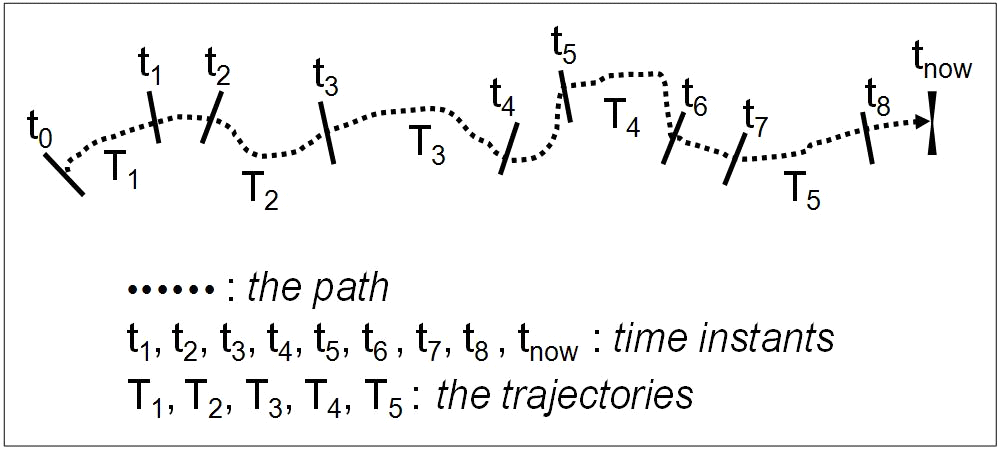
\includegraphics[scale=0.4]{pictures/trayectoria.png}
  \caption{Ruta Espacio Temporal \cite{spaccapietra2008conceptual}).}
  \label{fig:ruta}
\end{figure}

Para la Figura~\ref{fig:ruta}, una ruta espacio-temporal para un objeto en movimiento
en curso y sus muchas trayectorias definidas por una segmentación semántica de la ruta. En este ejemplo partes del
camino no pertenece a ninguna trayectoria, corresponden al movimiento que es irrelevante a la aplicación.
Los objetos que se desplazan no necesariamente se mueven continuamente durante una trayectoria. En consecuencia, las
trayectorias pueden ser ellas mismas segmentadas semánticamente mediante la definición de una secuencia temporal de
sub-intervalos de tiempo donde alternativamente la posición del objeto cambia y permanece fija. La primera se llama
movimiento y la segunda parada. Podemos ver entonces una trayectoria como una secuencia de movimientos que van de
una parada a la siguiente (o como una secuencia de paradas que separan los movimientos). Por ejemplo, un ave que se
ha apartado de la migración hará una parada en algún lugar durante algún tiempo para alimentarse, otra parada para
descansar, y así sucesivamente hasta que se alcanza el final de su trayectoria. Vendedores en viaje de negocios se
detendrán en todas las localidades donde planeaban encontrarse con un cliente.

Identificar paradas (y movimientos) dentro de una trayectoria es la responsabilidad de la aplicación. Paradas 
físicas (es decir, el hecho de que la posición del objeto es el mismo durante dos o más instantes consecutivos)
no se tienen en cuenta para las paradas conceptuales, ya que puede ser debido a eventos que son irrelevantes 
para la aplicación. Por ejemplo, la parada hecha por vendedor para beber un café es irrelevante para la
aplicación de seguimiento de la empresa. En su lugar, la parada de hecho para cumplir con 
un cliente es significativo. La aplicación podría estar interesado en contar el número 
de paradas por trayectoria, y, obviamente, las paradas que se cuentan son sólo las paradas
importantes. Se asume que se mueve y se para completamente para cubrir la trayectoria (es decir, 
no hay instante en [$t_{inicio}$, $t_{fin}$] que
no pertenezca ni a un movimiento ni a una parada).

Se definen semánticamente paradas y movimientos de la siguiente manera:

\begin{description}
 \item [Definición 2 (Parada)] Una parada es una parte de una trayectoria, de tal manera que:

El usuario ha definido explícitamente que es parte de la trayectoria ($[t_{inicioparadax}$, $t_{finparadax}]$) 
para representar una parada. La extensión temporal $[t_{inicioparadax}$, $t_{finparadax}]$ es un intervalo de tiempo
no vacía, y el objeto que se desplaza no se mueve (por lo que la vista de la aplicación de esta 
trayectoria se refiere), es decir, el rango espacial de la trayectoria para el intervalo 
$[t_{inicioparadax}$, $t_{finparadax}]$ es de un solo punto. Todas las paradas están temporalmente
disjuntas, es decir, la extensión temporal de dos paradas son siempre disjuntos.
\end{description}


\begin{description}
 \item [Definición 3 (Movimiento)] Un movimiento es una parte de una trayectoria, de tal manera que:

La parte está delimitada por dos extremidades que representan ya sea dos consecutivas paradas, o 
$t_{inicio}$ y la primera parada, o la última parada y $t_{fin}$, o $[t_{inicio}$, $t_{fin]}]$.

La extensión temporal $[t_{iniciomovimientox}$, $t_{finmovimientox}]$ es un intervalo de tiempo no vacía,y el 
rango espacial de la trayectoria para el intervalo $[t_{iniciomovimientox}$, $t_{finmovimientox}]$ es la línea 
espacio-temporal (no un punto) definido por la función de trayectoria (de hecho, es la línea poligonal 
construida sobre los puntos de muestreo en el intervalo $[t_{iniciomovimientox}$, $t_{finmovimientox}]$).
\end{description}


Desde el punto de vista de diseño de base de datos, un movimiento es un punto de tiempo variable 
definida en el intervalo de tiempo $[t_{iniciomovimientox}$, $t_{finmovimientox}]$. \cite{spaccapietra2008conceptual}

\section{IDENTIFICACIÓN DE PATRONES EN OBJETOS EN MOVIMIENTO}

Debido a la creciente disponibilidad de bases de datos espaciales, se han propuesto diferentes 
metodologías con el fin de encontrar información significativa que permanece oculta en este tipo de 
datos. Tratar de comprender cómo diversas entidades se mueven en un contexto espacial,  han 
demostrado ser útiles en temas tan diversos como el deporte \cite{iwase2004parallel}, la geografía 
socioeconómica \cite{frank2001life}, la migración de los animales \cite{dettki2004real} y la 
seguridad y la vigilancia \cite{makris2002path} \cite{piciarelli2006trajectory}. 

Los primeros enfoques de recuperación de información de bases de datos 
espacio-temporales incluyen para esto consultas destinadas a responder gama simple de predicado o 
consultas de vecinos más cercanos, por 
ejemplo, ``encontrar todos los objetos en movimiento dentro de la zona A entre las 10 a.m. a 
las 02:00 PM''  o "¿Cuántos coches condujeron entre la plaza principal y el aeropuerto el viernes". 
Extensiones de consultas espaciales en  paquetes comunes de software de SIG
y DBMS que son capaces de ejecutar este tipo de de consultas, sin embargo estas técnicas tratan de 
encontrar la mejor solución a explorar cada objeto espacial 
 a la vez de acuerdo con alguna métrica de distancia (por lo general euclidiana). Como 
resultados, es difícil de capturar el comportamiento colectivo y las correlaciones entre las 
entidades involucradas utilizando este tipo de consultas. 

Recientemente, han surgido unos nuevos intereses para la consulta de captura de patrones de ``grupo'' 
o conducta ``común'' entre las entidades en movimiento. De particular interés es el desarrollo 
de enfoques para identificar grupos de objetos en movimiento cuya participación en una relación 
fuerte y la interacción en una región espacial definida durante una duración de tiempo determinado. 
Algunos ejemplos de este tipo de enfoques son movimiento de cluster \cite{kalnis2005discovering} 
\cite{jensen2007continuous}, consultas de convoy \cite{jeung2008discovery-1} y patrones de 
agrupamiento \cite{gudmundsson2006computing} \cite{benkert2008reporting} \cite{VieiraT13} 
\cite{turdu2014}. 

Aunque diferentes interpretaciones pueden ser tomadas, un patrón de agrupamiento se refiere a un 
número predefinido de entidades que permanecen lo suficientemente cerca durante al menos un 
intervalo de tiempo dado. El desafiar a identificar este tipo de patrones de movimiento es 
especialmente relevante debido a la interacciones intrínsecas entre los miembros del grupo, 
especialmente en el contexto de los animales, peatones o vehículos. En esta investigación un marco 
alternativo para descubrir en movimiento  acuden patrones se propone. Esta investigación esta 
basada en un algoritmo existente denominado BFE propuesto por \cite{VieiraT13}, y otro 
llamado LCMFlock propuesto \cite{turdu2014} el cual extiende el algoritmo de BFE tomando ventaja de 
algoritmos de patrones frecuentes de minería en el area del aprendizaje de reglas de asociación.


\section{PATRÓN DE AGRUPAMIENTO}

\cite{vieira2009line} 
define patrones de agrupamiento también conocidos como flocks, como el problema de 
identificar todos los grupos 
de trayectorias que permanecen
``juntas'' por la duración de un intervalo de tiempo dado. Se Considera que los objetos en 
movimiento están suficientemente
cerca si existe un disco con un
radio dado que cubre todos los objetos que se mueven en el patrón 
(figura~\ref{fig:flockexample}). Una trayectoria satisface el 
patrón anterior, siempre y cuando suficientes trayectorias están contenidos 
dentro del disco para el intervalo de
tiempo especificado, es decir, la respuesta se basa no sólo en el comportamiento 
de una trayectoria dada, sino
también en las más cercanas a ella. Uno de los enfoques para descubrir patrones 
móviles de agrupamiento consiste
en encontrar un conjunto adecuado de discos en cada instante de tiempo y luego 
combinar los resultados de un 
instante de tiempo a otro. Como consecuencia, el rendimiento y el número de 
patrones encontrados depende del número
de los discos y cómo éstos se combinan.

En el ejemplo de la figura~\ref{fig:flockexample}, se muestra un patrón de 
agrupamiento el cual contiene tres 
trayectorias (T1, T2 y T3)
que están dentro de un disco en tres instantes de tiempo consecutivos. Los 
discos se pueden
mover libremente en el espacio bidimensional con el fin de acomodar los tres 
objetos en movimiento  y su centro no necesariamente
tiene que ser la localización de alguno de los objetos. Esto hace que el
descubrimiento de patrones sea mucho más complicada  porque hay un número 
infinito de posibles
colocaciones del disco en cualquier instante de tiempo y el posible número de 
combinaciones puede llegar a ser muy alta y costosa.

\begin{figure}
  \centering
  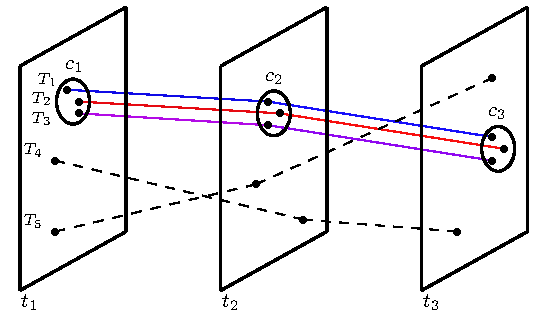
\includegraphics[scale=0.8]{pictures/flock_example.pdf}
  \caption{Ejemplo de patrones de agrupamiento \cite{vieira2009line}.}
  \label{fig:flockexample}
\end{figure}


\section{BFE (BASIC FLOCK EVALUATION)}

Este algoritmo en línea presentado por \cite{VieiraT13}, al parecer es el primer trabajo que 
presenta una solución exacta para reportar patrones de agrupamiento (flocks) en tiempo polinomial.

Un patron de agrupamiento Flock($\mu, \varepsilon, \delta$), esta definido de la siguiente manera:


\textbf{Definición:}  Dado un conjunto de trayectorias $\tau$ , un mínimo número de trayectorias 
$\mu >1 (\mu \in N)$, una máxima distancia $\epsilon > 0$ definida sobre la función de distancia d, 
y una duración de tiempo mínimo $\delta > 1 (\delta \in N)$. Un patron de agrupamiento
Flock($\mu, \epsilon, \delta$) reporta todas las colecciones máximas de tamaño F de 
trayectorias donde: para cada $f_{k}$ en F, el número de trayectorias en 
$f_{k}$ es mayor o igual que $\mu (|f_{k} | \geq \mu)$ y existen instancias de tiempo consecutivos 
$\delta$ 
tal que para cada $t_{i} \in [f_{k}^{t_{1}} ..f_{k}^{t_{1} + \delta} ]$,
hay un disco con centro $c_{k}^{t_{i}}$ y el radio $\epsilon / 2$ que cubre todo 
los puntos en $f_{k}^{t_{i}}$. Es decir: 
$\forall f_{k} \in F, \forall t_{i} \in [f_{k}^{t_{1}} ..f_{k}^{t_{1} + \delta}], \forall T_{j} \in 
f_{k}:  |f_{k}^{t_{i}}| \geq \mu, d(p_{j}^{t_{i}}, c_{k}^{t_{i}}) \leq \epsilon /2$

\section{PATRONES FRECUENTES EN BASE DE DATOS TRADICIONALES}

Patrones frecuentes son conjuntos de elementos, subsecuencias, o subestructuras que aparecen en un conjunto de datos con una
frecuencia no inferior a un umbral especificado por el usuario \cite{han2007frequent}. La cuestión de las modalidades 
interesantes desvelando en las bases de datos en diferentes contextos ha sido un tema de investigación
recurrente durante los últimos 15 años. Minería de datos general ha sido ampliamente reconocido como un
crítico campo por empresas de todo tipo. Como parte de los métodos de minería de datos, la tarea de aprendizaje 
de reglas de asociación han estudiado diferentes algoritmos de minería de patrones frecuente de identificar tendencias relevantes en los conjuntos de datos en diferentes disciplinas \cite{creighton2003mining} \cite{miller2009geographic} \cite{zhang2002association}. 

Una de las áreas en las que las técnicas de aprendizaje de reglas de asociación y el patrón frecuente 
algoritmos de minería se han aplicado con más frecuencia en el análisis de datos y tendencias del
mercado en transacciones de clientes de grandes supermercados y tiendas \cite{agrawal1994fast}. Por lo general, esta técnica 
tiene dado el nombre del problema de la cesta de compras a pesar de que los métodos derivados de resolverlo puede ser aplicado en diferentes contextos \cite{han2006data}.

El problema de la cesta de compras representa un intento por parte de un minorista para descubrir qué 
artículos de sus clientes compran con frecuencia juntos \cite{tsur1998query}. El objetivo es la comprensión de la 
comportamiento de un cliente típico y la identificación de los objetos de valor y relaciones 
entre ellos. Para este tipo de problema de la entrada es una base de datos con la información dada 
acerca de los artículos comprados. Cuando un cliente paga por sus productos en el cajero, un registro 
con los artículos comprados se inserta en la base de datos. En una vista general, es suficiente para 
capturar sólo el ID de la transacción y la identificación del producto (un registro por cada artículo comprado). 
Se le conoce como {TID: conjunto de elementos} esquema. Como los registros de la base de datos por lo general se refieren a 
transacciones, estas bases de datos se denominan bases de datos transaccionales. El objetivo de las compras 
análisis de la cesta es encontrar conjuntos de elementos (conjuntos de elementos) que están ``asociados'' y el hecho de 
su asociación a menudo se llama una regla de asociación \cite{tsur1998query}. 

Por ejemplo, si se sabe que un alto porcentaje de clientes están comprando leche y pan 
al mismo tiempo, en sus visitas a un supermercado, esta relación representa una regla de asociación. Se puede 
utilizar para formular nuevas estrategias de marketing, promociones, introducción de 
nuevos productos, diseño de catálogo, cruces de marketing o planificación de espacio en las
estanterías \cite{han2006data}. Es habitual localizar elementos asociados en diferentes pasillos y de alta rentabilidad
o nuevos productos entre ellos para asegurarse de que están expuestos a más clientes \cite{tsur1998query}. \cite{giudici2005applied} analizan 
otros casos de estudio aplicados en el comercio y el marketing, donde se exploran métodos diferentes reglas
de asociación. durante los últimos años muchas mejoras y nuevas técnicas se han desarrollado y propuesto 
con el fin de mejorar y tomar ventaja de los beneficios del análisis de reglas de asociación.

\section{LCM (LINEAR TIME CLOSED ITEMSET MINER)}

El problema de LCM propuesto por \cite{uno2005lcm} se define de la siguiente manera.

Sea I un conjunto de elementos. Sea D una base de datos transaccional de tal manera que cada 
registro (llamada transacción) es un conjunto de elementos. La frecuencia de un conjunto de 
elementos es el número de transacciones, incluyendo el conjunto de elementos. Para un número dado t 
(llamado soporte), un conjunto de elementos se dice que es frecuente si su frecuencia es no menos de 
t. Un conjunto de elementos frecuente se llama máxima si está incluido en ningún otro conjunto de 
elementos frecuentes, y se llama cerrada si está incluido en ningún otro conjunto de elementos de la 
misma frecuencia. La tarea de LCM, es enumerar (sacar, o contar) todos los conjuntos de elementos 
frecuentes, todos los conjuntos de elementos frecuentes máximos, o todos los conjuntos de elementos 
frecuentes cerrados en una base de datos transaccional para un soporte dado.
% \chapter{TRABAJOS RELACIONADOS}

Las capacidad de recolectar datos de objetos en movimiento ha ido aumentando 
rápidamente y el interés de consulta
de patrones que describen el comportamiento colectivo también ha aumentado. 
\cite{vieira2009line} enumera tres grupos de patrones
``colectivos'' en bases de datos de objetos en movimiento: clústers móviles, 
consulta de convoyes y patrones de agrupamiento.

Los clústers móviles \cite{jensen2007continuous} \cite{kalnis2005discovering} 
\cite{li2008mining} 
y  consultas de convoyes  \cite{jeung2008discovery-1} \cite{jeung2008convoy}, 
tienen en común que se basan en algoritmos
de clústering, principalmente en algoritmos basados en densidad como el 
algoritmo DBSCAN\cite{ester1996density}.

Los clústers móviles se definen entre dos instantes de tiempo consecutivos. Los 
clústers  se pueden unir sólo si el número de objetos comunes entre ellos están 
por encima del parámetro predefinido.
Un clúster es reportado si no hay otro nuevo clúster que pueda ser unido a éste. 
Este proceso se aplica cada vez para 
todos los instantes de tiempo en el conjunto de datos. 

Las consultas de convoyes se definen como un clúster denso de trayectorias que 
permanecen juntas al menos por un tiempo contínuo predefinido. 

Las principales diferencias entre las dos técnicas son la forma en que se unen 
los grupos  entre dos intervalos
consecutivos de tiempo y el uso de un parámetro adicional para especificar un 
tiempo mínimo de duración. Aunque
estos métodos están estrechamente relacionados con los patrones de agrupamiento, 
ninguno de ellos asume una  forma predefinida.

Previos trabajos de detección de patrones de agrupamiento móviles son descritos 
por \cite{ gudmundsson2006computing}
y \cite{benkert2008reporting}. Ellos introducen
el uso de discos con un radio predefinido para identificar  grupos de 
trayectorias que se mueven juntos en la misma
dirección, todas las trayectorias que se encuentran dentro del disco en un 
instante  de tiempo particular se 
considera un patrón candidato. La principal limitación de este proceso es que 
hay un número infinito de posibles
ubicaciones del disco en cualquier instante de tiempo. En efecto, en 
\cite{gudmundsson2006computing} se ha demostrado
que el descubrimiento de agrupaciones fijas, donde los patrones de las mismas 
entidades permanecen juntas durante 
todo el intervalo, es un problema NP-complejo. 

\cite{vieira2009line} son  los  primeros  en  presentar  una  solución  exacta  
para  reportar  patrones  de agrupación en tiempo polinomial, y también pueden trabajar efectivamente en 
tiempo real. Su trabajo revela que el tiempo de solución polinomial se puede encontrar 
a través de  la  identificación  de  un  número  discreto  de  ubicaciones  para  colocar 
 el  centro  del disco.  Los  autores  proponen  el  algoritmo  BFE  (Basic  Flock  Evaluation)  
basado  en  el tiempo de unión y combinación de los discos. La idea principal de este algoritmo 
es primero  encontrar  el  número  de  discos  válidos  en  cada  instante  de  
tiempo  y  luego combinarlos  uno  a  uno  entre  tiempos  adyacentes. Adicionalmente,  se  
proponen  otros cuatro  algoritmos  basados  en  métodos  heurísticos,  para  reducir  el  
número  total  de candidatos  a  ser  combinados  y,  por  lo  tanto,  el  costo  global del
algoritmo.  Sin  embargo,  el pseudocódigo y  los  resultados  experimentales
muestran todavía una alta complejidad computacional, largos tiempos de respuesta,
debido a que este algoritmo usa $\delta$ para partir los flocks hace que el número de patrones
encontrados sea mayor y esto hace difícil su interpretación.


\cite{romero2011mining} y \cite{turdu2014} proponen  una  metodología  que  
permite  identificar  patrones de agrupamiento utilizando tradicionales y potentes algoritmos de minería de datos 
usando patrones frecuentes, el cual fue comparado con BFE demostrando un alto 
rendimiento con conjuntos de datos sintéticos, aunque con conjuntos de datos reales el 
tiempo de respuesta siguió siendo eficiente pero similar a BFE. Este algoritmo trata el 
conjunto de trayectorias como una base de datos transaccional al convertir cada trayectoria, 
que se define  como  un  conjunto  de  lugares  visitados,  en  una  transacción,  
definida  como  un conjunto  de ítems.  De  esta  manera,  es  posible  aplicar  cualquier  
algoritmo  de  reglas  de asociación y encontrar patrones frecuentes sobre el conjunto dado, este algoritmo hace un llamado a LCM
propuesto por \cite{uno2004lcm} para encontrar patrones máximos y eso permite encontrar los flocks más largos.
%  
\chapter{METODOLOGÍA}

Para poder realizar esta investigación, primero se realizó una apropiación de 
conocimiento y se definió el marco conceptual sobre el cual se iba a realizar el proyecto. Primero fue importante 
entender el problema que se desarrollaría, identificando los patrones en objetos en movimiento, 
para posteriormente enfocarse en los patrones de agrupamiento conocidos como ``flocks''.

Se compararon dos algoritmos, BFE y LCMFlock propuestos por \cite{VieiraT13} y \cite{turdu2014}, con el fin de
identificar los problemas asociados a su rendimiento. Se escogió únicamente estos dos algoritmos 
para la comparación debido a que este análisis se enfocaría únicamente a patrones de agrupamiento 
(flocks) y estos son los algoritmos más representativos que existen hasta
el momento en este campo. 

Para realizar esta comparación se implementaron los algoritmos BFE y LCMFLOCK basados en el 
pseudo-código publicado por \cite{vieira2009line}  y \cite{romero2011mining} respectivamente,
usando Python versión 3 debido a la facilidad y comodidad para el programador. 
Realizar esta implementación tenía como objetivo hacer una inspección más detallada de cada 
algoritmo y de las estructuras utilizadas en la implementación con el fin de encontrar
sus inconvenientes y buscar una mejora. El código fuente se  puede descargar
desde el repositorio del proyecto \footnote{Repositorio del proyecto: 
\url{https://github.com/poldrosky/FPFlock}}.

A continuación se describen los detalles de la implementación de los algoritmos BFE y LCMFlock.

\section{IMPLEMENTACIÓN DE BFE}

Este algoritmo se divide en dos partes: la primera parte, encontrar los discos 
dado un radio ($\epsilon$) y un número mínimo de puntos ($\mu$) para cada instante de tiempo. La 
segunda parte, encontrar
el número de puntos que permanecen juntos (flocks) durante un rango de tiempo ($\delta$).

Para la primera parte es necesaria la utilización tanto de diccionarios de datos como
estructuras kd-tree para la búsqueda del vecino más cercano, en esta implementación se usó la clase 
scipy.spatial.cKDTree de
SciPy \footnote{Scipy es un ecosistema basado en Python, software de código abierto para las 
matemáticas, la ciencia y la ingeniería.
\url{http://www.scipy.org/}} la cual proporciona  un índice dentro de un conjunto de puntos 
k-dimensionales que se pueden utilizar
para buscar rápidamente los vecinos más cercanos de cualquier punto. 

Para realizar este proceso de implementación fue de gran utilidad el uso del software QGIS, un 
sistema de información geográfica libre y de código abierto disponible en \cite{QGISsoftware}, 
debido a que la primera parte del algoritmo esta basada en encuentrar de los discos máximos, se 
utilizo QGIS para realizar pruebas unitarias a medida que se avanzaba en las etapas de 
depuración, como lo muestra la figura~\ref{fig:findMaximalDisk}.

\begin{figure*}
  \centering
  \subfigure[Todos los discos]{\label{b1} 
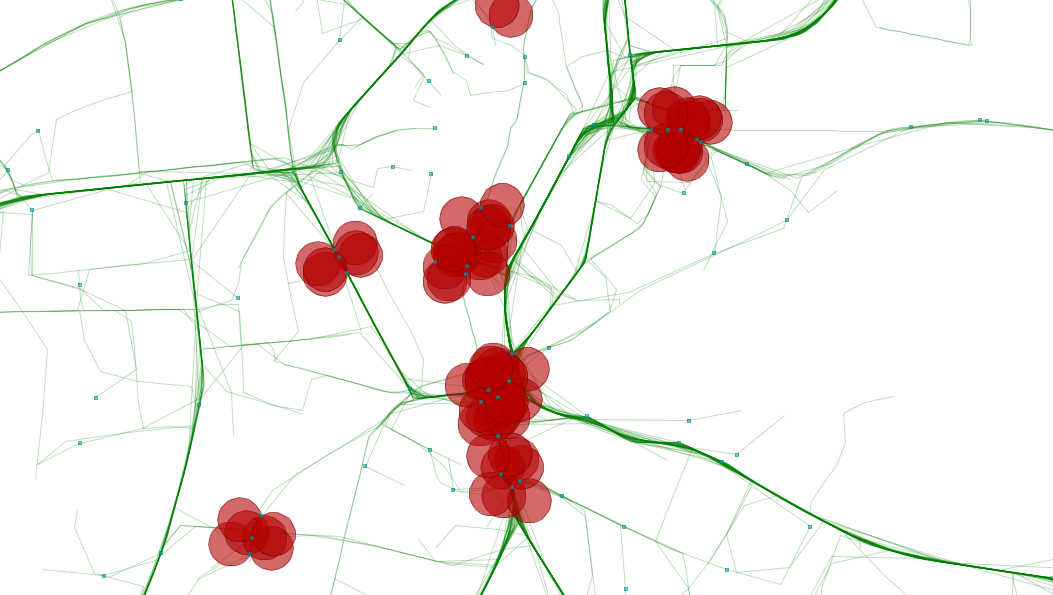
\includegraphics[scale=0.3]{pictures/bfe1.png}}
  \subfigure[Discos que cumplen $\mu$ mínimo]{\label{b2} 
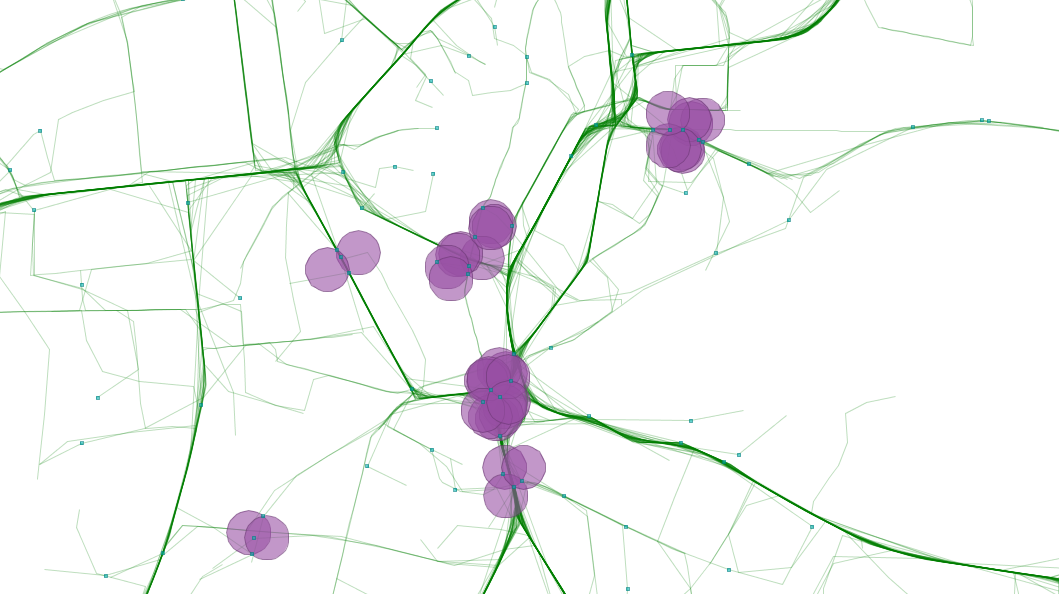
\includegraphics[scale=0.3]{pictures/bfe2.png}}
\subfigure[Discos máximos]{\label{b3} 
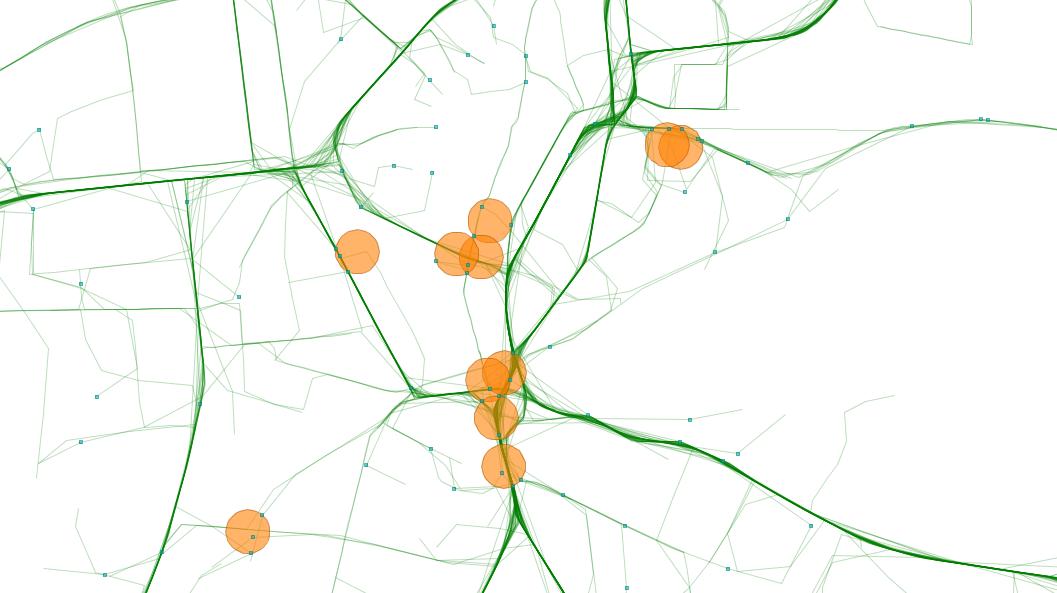
\includegraphics[scale=0.3]{pictures/bfe3.png}}
  \caption{Proceso para encontrar los discos máximos \cite{romero2011mining}.}
  \label{fig:findMaximalDisk}
\end{figure*}


Los conjuntos de discos para 
cada instante de tiempo se almacenaron en diccionarios los cuales fueron combinados en la segunda 
parte del algoritmo.  Finalmente, se almacenaron en una base de datos los flocks que cumplían los 
parámetros solicitados.  Para cada flock se almacenó un arreglo con los objetos que pertenecen a 
dicho flock, y los tiempos de inicio y final para cada caso.


\section{IMPLEMENTACIÓN DE LCMFLOCK}

Este algoritmo usa la primera parte del algoritmo de BFE para encontrar los discos. En la segunda 
parte, para abordar el problema
de combinatoria utiliza un enfoque de patrones frecuentes, en el cual se construyó un 
diccionario de datos asociando la localización 
de los puntos de cada trayectoria con su respectivo disco generado una versión transaccional del 
conjunto de datos. En la figura~\ref{fig:transactionTrajectory}, se muestra como se realiza conversión de las trayectorias en  
transacciones. Este conjunto
es pasado como parámetro, junto con el  número mínimo de puntos ($\mu$), al algoritmo 
LCM\cite{uno2004lcm}, disponible para descargar en \cite{FIMIHomep}.

\begin{figure*}
  \centering
  \subfigure[\cite{romero2011mining}]{ 
  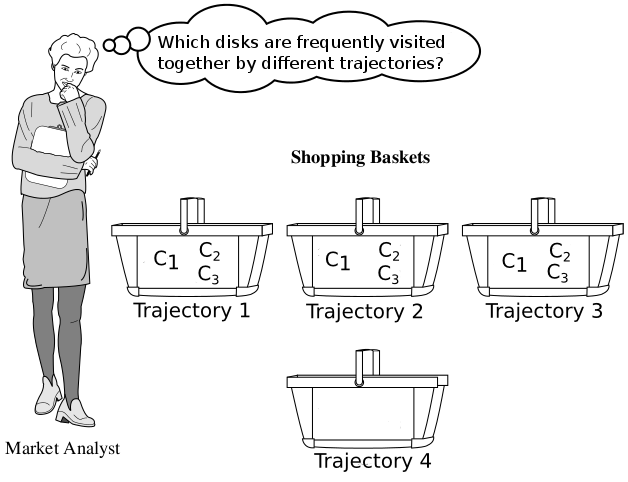
\includegraphics[scale=0.5]{pictures/lcm2.png}}
  \subfigure[\cite{vieira2009line}]{
  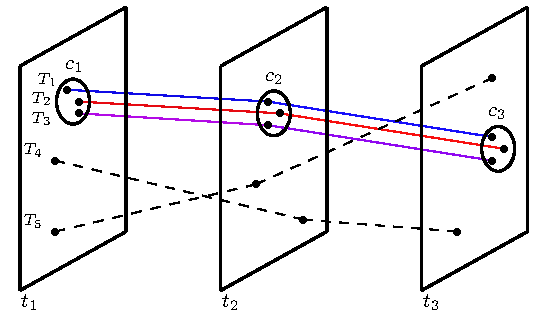
\includegraphics[scale=0.8]{pictures/flock_example.pdf}}
  \caption{Ejemplos de patrones frecuentes en trayectorias.}
  \label{fig:transactionTrajectory}
\end{figure*}

 Aquí se encuentran disponibles dos variantes del programa; LCM\_max y LCM\_closed los cuales 
recuperarán el conjunto de patrones máximo y cerrado\cite{han2000mining}.  LCMFLOCK utiliza el 
concepto de patrones máximos y cerrados para identificar los patrones de agrupamiento de mayor 
duración.  De esta manera, el parámetro $\delta$ se utiliza solo para filtrar aquellos patrones que 
no cumplan con este parámetro \cite{romero2011mining}.
 
 La salida de LCM es un archivo de texto, donde cada línea es un patrón que contiene un conjunto de 
ID's de discos separados por espacios que representan los patrones de agrupamiento (flocks). Sin 
embargo, se requiere de un análisis posterior para verificar que dichos discos ocurran en tiempos 
consecutivos.  De cada patrón, se extraen los objetos que encierra cada disco así como los tiempos 
de inicio y final los cuales son almacenados en una base de datos.
 
\section{VALIDACIÓN}
 
 Para poder validar la correcta implementación de los algoritmos se siguió una metodología similar a 
la propuesta en \cite{benkert2008reporting}. Se crearon conjuntos de datos sintéticos a los cuales 
se les insertó aleatoriamente un número específico de trayectorias y flocks. La 
tabla~\ref{tab:validacion}, relaciona los conjuntos de datos construidos y con los cuales los 
algoritmos fueron validados.  Una copia de los conjuntos de datos y el script utilizado para la 
validación está disponible en el repositorio del proyecto \footnote{Conjuntos de prueba: 
\url{https://github.com/poldrosky/FPFlock/tree/master/Src/Datasets/}}. El total de flocks insertados 
en cada caso fueron correctamente descubiertos por las dos implementaciones.
 
\begin{table}
\caption{Conjunto de datos validación}
\label{tab:validacion}
\centering
\scalebox{0.8}{
\begin{tabular}{c c r r c}
\toprule
\multirow{2}{*}{Dataset}& \multirow{2}{*}{Red}& \multicolumn{1}{c}{Número de}& Número de  & 
Instantes de\\
                        &                         & Trayectorias & \multicolumn{1}{c}{Flocks} & 
tiempo\\
\midrule
SJ5000T100t100f  & Sintética & 5000 & 100 & 100 \\
SJ5000T100t200f	& Sintetica & 5000 & 200 & 100 \\
SJ5000T100t300f	& Sintetica & 5000 & 300 & 100 \\
SJ5000T100t400f	& Sintetica & 5000 & 400 & 100 \\
SJ5000T100t500f	& Sintetica & 5000 & 500 & 100 \\
SJ2500T100t500f  & Sintética & 2500 & 500 & 100  \\
SJ7500T100t500f  & Sintética & 7500 & 500 & 100  \\
SJ10000T100t500f  & Sintética & 10000 & 500 & 100  \\
SJ12500T100t500f  & Sintética & 12500 & 500 & 100  \\
SJ15000T100t500f  & Sintética & 15000 & 500 & 100  \\
SJ17500T100t500f  & Sintética & 17500 & 500 & 100  \\
SJ20000T100t500f  & Sintética & 20000 & 500 & 100  \\
\bottomrule
\end{tabular}}\par
\bigskip
\end{table}

\section{ANÁLISIS DE BFE y LCMFLOCK}

Se realizó un análisis de desempeño entre los algoritmos de BFE y LCMFLlock, usando varios 
conjuntos de prueba, este análisis se puede detallar en \cite{cabrera}. Algunas de las 
conclusiones de este análisis, fueron:

\begin{itemize}
\item Las estructuras de tipo árbol, y en específico, los kd-tree presentaron los mejores 
resultados. Esto se configura
como un aspecto clave para la búsqueda del conjunto final
de discos para cada instante de tiempo. 

 \item Aunque el proceso de identificación de los discos en cada
instante de tiempo es compartido por ambos algoritmos, el
proceso de combinación es mucho más eficiente utilizando
un enfoque basado en técnicas de patrones frecuentes.

\item Aunque LCMFLock presenta mejores resultados, este
aún se ve afectado por el proceso de identificación de los
discos. El número de discos a evaluar crece exponencialmente a medida que crece el valor $\varepsilon$ de y la 
densidad de puntos dentro del conjunto.

\item En BFE, el reporte de flocks es demasiado alto en
comparación con LCMFlock. BFE separa los
flocks de acuerdo al parámetro $\delta$ en procura de limitar
el número de discos a comparar. Esto dificulta la interpretación de resultados ya que es necesario 
de un análisis adicional para encontrar los flocks más largos a partir de
aquellos con una duración fija. En LCMFlock esto se
soluciona con el uso del algoritmo LCM para la detección
de patrones máximos y cerrados.

\item La capacidad de encontrar los flocks más largos ciertamente es una ventaja de LCMFlock sobre 
BFE. Sin embargo, LCMFlock, a diferencia de BFE, requiere de
una ventana fija de tiempo donde será aplicado lo que
le impide reportar patrones en tiempo real. 
\end{itemize}

Debido a este análisis realizado el algoritmo propuesto, presentado en el siguiente capítulo se 
enfocó en resolver dos problemas claves: mejorar el desempeño
durante la búsqueda de los discos e implementar mecanismos de detección en tiempo real.





% \chapter{ALGORITMO FP-FLOCK}

En el algoritmo propuesto por \cite{VieiraT13}, en la primera parte del algoritmo se encuentra el total de discos con los 
objetos móviles que están juntos, se eliminan discos que no cumplan $\mu$, este proceso genera que se encuentren varios de
 los discos solapados, para ello, por último, se realiza una limpieza de los discos solapados haciendo iteraciones en los discos
 encontrados y dejando únicamente aquellos discos con mayor número de miembros denominados discos máximos, este proceso de
 limpieza de los discos solapados hace que el costo computacional sea muy alto debido a la cantidad de iteraciones. En la 
segunda parte, el algoritmo realiza un proceso de combinación para el descubrimiento de flocks en el cual si el $\varepsilon$ aumenta
 el algoritmo puede llegar a colapsar. Este algoritmo separa los flocks de acuerdo al parámetro $\delta$ en procura de limitar
 el número de discos a comparar, esto dificulta la interpretación de resultados ya que es necesario de un análisis adicional 
para encontrar los flocks más largos a partir de aquellos con una duración fija.

Para el algoritmo propuesto por \cite{romero2011mining}, ya que usa la primera parte del algoritmo en \cite{VieiraT13}, tiene 
el mismo problema de los discos solapados. Ya en la segunda parte, al tratar el proceso de combinación es mucho más
eficiente ya que utiliza un enfoque basado en técnicas de patrones frecuentes, aunque con la desventaja que el proceso se 
realiza en una ventana fija  de tiempo  lo que le impide reportar patrones en tiempo real. 

La alternativa propuesta resuelve los problemas que poseen los algoritmos anteriores utilizando patrones frecuentes, se proponen 
el algoritmo llamado FP-Flock con dos variaciones, uno fuera de línea y otro en tiempo real.


\section{FP-FLOCKOFFLINE}

En la primera parte se hace el cálculo de los discos máximos, para lo cual se tomó como base el algoritmo 1 propuesto
 por \cite{VieiraT13} al cual se le hicieron modificaciones para hacer una limpieza de los discos solapados usando 
patrones frecuentes de minería. Puntualmente, se usó el algoritmo LCM \cite{uno2005lcm}. El pseudo-código de la primera
 parte del algoritmo es presentado en Algoritmo~\ref{alg:maximalDisks}. 

\begin{algorithm}
    \renewcommand{\algorithmicrequire}{\textbf{Input:}}
    \renewcommand{\algorithmicensure}{\textbf{Output:}}
    \renewcommand{\algorithmicprint}{\textbf{break}}
  \caption{Computing maximal disks.}
  \label{alg:maximalDisks}
  \algsetup{indent=2em}
  \footnotesize
  \begin{algorithmic}[1]
\REQUIRE {set of points $T[t_i]$ for timestamp $t_i$} 
\ENSURE {sets of maximal disks $C$}
\STATE $C \leftarrow \emptyset$
\STATE Index.Build($T[t_i],\varepsilon)$ \COMMENT{call Algorithm 1 in \cite{VieiraT13}}
\FOR {each non-empty cell $g_{x,y} \in$ Index}
  \STATE {$L_r \leftarrow g_x,_y$} 
  \STATE {$L_s \leftarrow [g_{x-1,y-1}... g_{x+1,y+1}]$}
  \IF {$|L_s| \geq \mu$}
    \FOR {each $l_r \in L_r$}
      \STATE {$H \leftarrow Range(l_r, \varepsilon), |H| \geq \mu, d(l_r,l_s) \leq \varepsilon, l_s \in L_s $}
      \FOR {each $l_j \in H$}
	\IF{ $\{l_r, l_j\}$ not yet computed}
	  \STATE {compute left disk $\{c\}$ defined by ${l_r, l_j}$ and diameter $\varepsilon$}
	  \STATE {D $\leftarrow$ points $\in c$ }
	\ENDIF
      \ENDFOR
    \ENDFOR
  \ENDIF
  \STATE $min\_sup \leftarrow 1$ 
  \STATE {C $\leftarrow$ call $LCM\_max(D, min\_sup)$  \COMMENT{call LCM Algorithm \cite{uno2005lcm}}}
\ENDFOR
\end{algorithmic}
\end{algorithm}

El algoritmo fuera de línea, se construyó usando el pseudo-código propuesto en \cite{turdu2014}, pero utilizando el algoritmo descrito anteriormente.

\section{FP-FLOCKONLINE}

El algoritmo en tiempo real, hace modificaciones al algoritmo propuesto en \cite{turdu2014},
este algoritmo en su primera parte usa el Algoritmo~\ref{alg:maximalDisks}, para solucionar el problema de los discos solapados.
En su segunda parte, se va liberando memoria en cada transacción, teniendo en cuenta las trayectorias que en ese 
instante de tiempo tuvieron un corte. En este algoritmo por cada intervalo de tiempo se realiza un llamado al 
algoritmo LCM propuesto por \cite{uno2005lcm} con el objetivo de reportar los patrones obtenidos hasta el momento.

El pseudo-código  del algoritmo en tiempo real es presentado en Algoritmo~\ref{alg:framework2}


\begin{algorithm}
    \renewcommand{\algorithmicrequire}{\textbf{Input:}}
    \renewcommand{\algorithmicensure}{\textbf{Output:}}
    \renewcommand{\algorithmicprint}{\textbf{break}}
  \caption{FP-FlockOnline: Frequent pattern flock  online.}

  \label{alg:framework2}

  \algsetup{indent=2em}

  \footnotesize

  \begin{algorithmic}[1]

\REQUIRE parameters $\mu$, $\varepsilon$ and $\delta$,
set of points $T$ 

\ENSURE flock patterns $F$
  \FOR{each new time instance $t_i \in T$}
    \STATE $C \leftarrow$ call $Index.Disks(T[t_i])$ \COMMENT{call Algorithm 1 in this paper}    
    \FOR{each $c_i \in C$}
      \STATE $P \leftarrow c_i.points$ 
      \FOR{each $p_i \in P$}
	  \STATE $c_i.time \leftarrow t_i$
	  \STATE $D[p_i] \leftarrow $ add $c_i.id$
      \ENDFOR
      \FOR {each $p_i \in P$}
	\IF {$D[p_i$] not was updated}
	    \STATE delete $D[p_i]$
	  \ENDIF
      \ENDFOR
    \ENDFOR
  \STATE $min\_sup \leftarrow \mu$
  \STATE $M \leftarrow$ call $LCM\_max(D,min\_sup)$ \COMMENT{call LCM Algorithm \cite{uno2005lcm}}
  \FOR{ each $max\_pattern \in M$}
  \STATE $id_0 \leftarrow max\_pattern[0]$
  \STATE $c_0 \leftarrow C[id_0]$
  \STATE $u \leftarrow c_0.points$
  \STATE $u.t_{start} \leftarrow c_0.time$
  \STATE $n \leftarrow max\_pattern.size$ 
  \FOR{$i=1$ \TO $n$}
	\STATE $id_i \leftarrow max\_pattern[i]$
	\STATE $c_i \leftarrow C[id_i]$
	\IF{$c_i.time = c_{i-1}.time + 1$} 
	  \STATE $u \leftarrow u \cap c_i.points$
	  \STATE $u.t_{end} \leftarrow c_i.time$
	\ELSE
	  \IF{$u.t_{end} - u.t_{start} > \delta$ \AND $u \notin F$}
		\STATE $F \leftarrow$ add $u$
		\STATE $u.t_{start} \leftarrow c_i.time$
	  \ENDIF
	\ENDIF
  \ENDFOR
  \IF{$u.t_{end} - u.t_{start} > \delta$ \AND $u \notin F$}
	\STATE $F \leftarrow$ add $u$
  \ENDIF
\ENDFOR
\ENDFOR

\end{algorithmic}

\end{algorithm}

\section{VALIDACIÓN}
 
Para poder validar la correcta implementación de los algoritmos se realizó el mismo proceso de  
validación mencionado en el capítulo anterior, con la implementación de BFE y LCMFlock, posterior a 
ello se realizó un proceso de validación visual.  

Para realizar una validación visual se utilizó el conjunto de datos de Oldenburg disponible en \cite{Brin:2010:Online}, el cual proporciona un conjunto de ejemplos y 
recursos que pueden ser utilizados en la demostración en línea o 
versión descargable del generador. Para empezar, se utilizó un conjunto de datos relativamente pequeña posición de 1.000 objetos en movimiento 
al azar en la ciudad alemana de Oldenburg. Los datos de la red (bordes y nodos) están disponibles en el sitio web. La simulación de datos recoge la latitud y longitud de los puntos generados durante 140 intervalos 
de tiempo. El número total de ubicaciones almacenadas es 57.016 puntos. Con este conjunto se construyeron mapas con las representaciones lineales de 
los flocks resultantes como lo muestra la tabla~\ref{tab:validacionOldenburg} con las cuatro implementaciones.
En la figura~\ref{fig:validation} se muestran los flocks obtenidos con los parámetros $\varepsilon$=300, $\mu$=3 y $\delta$=3 sobre el conjunto Oldenburg.
Estos mapas se los comparó usando un 
módulo que implementa la similitud estructural métrica de imagen (SSIM) 
\cite{Zhou2004}. Los resultados de la comparación muestran que todos los mapas son 
idénticos, y por lo tanto, los mismos flocks son reportados por los diferentes 
algoritmos.


\begin{table*}
\caption{Número de flocks generados por los algoritmos en el conjunto de Oldenburg $\mu$=3, $\delta$=3}
\label{tab:validacionOldenburg}
\centering
\begin{tabular}{c c r r c}
\toprule
$\varepsilon(m)$& BFE & LCM & FP-FlockOnline & FP-FlockOffline \\  

\midrule
50 & 131 & 27 & 150 & 27 \\
100 & 639 & 109 & 663 & 109 \\
150 & 1135 & 247 & 1226 & 247 \\
200 & 2755 & 523 & 2683 & 523 \\
250 & 5423 & 1150 & 6877 & 1150 \\
300 & 11196 & 2365 & 16671 & 2365 \\
\bottomrule
\end{tabular}\par
\bigskip
Fuente: Esta investigación.
\end{table*}


\begin{figure}
  \centering
  \subfigure[BFE]{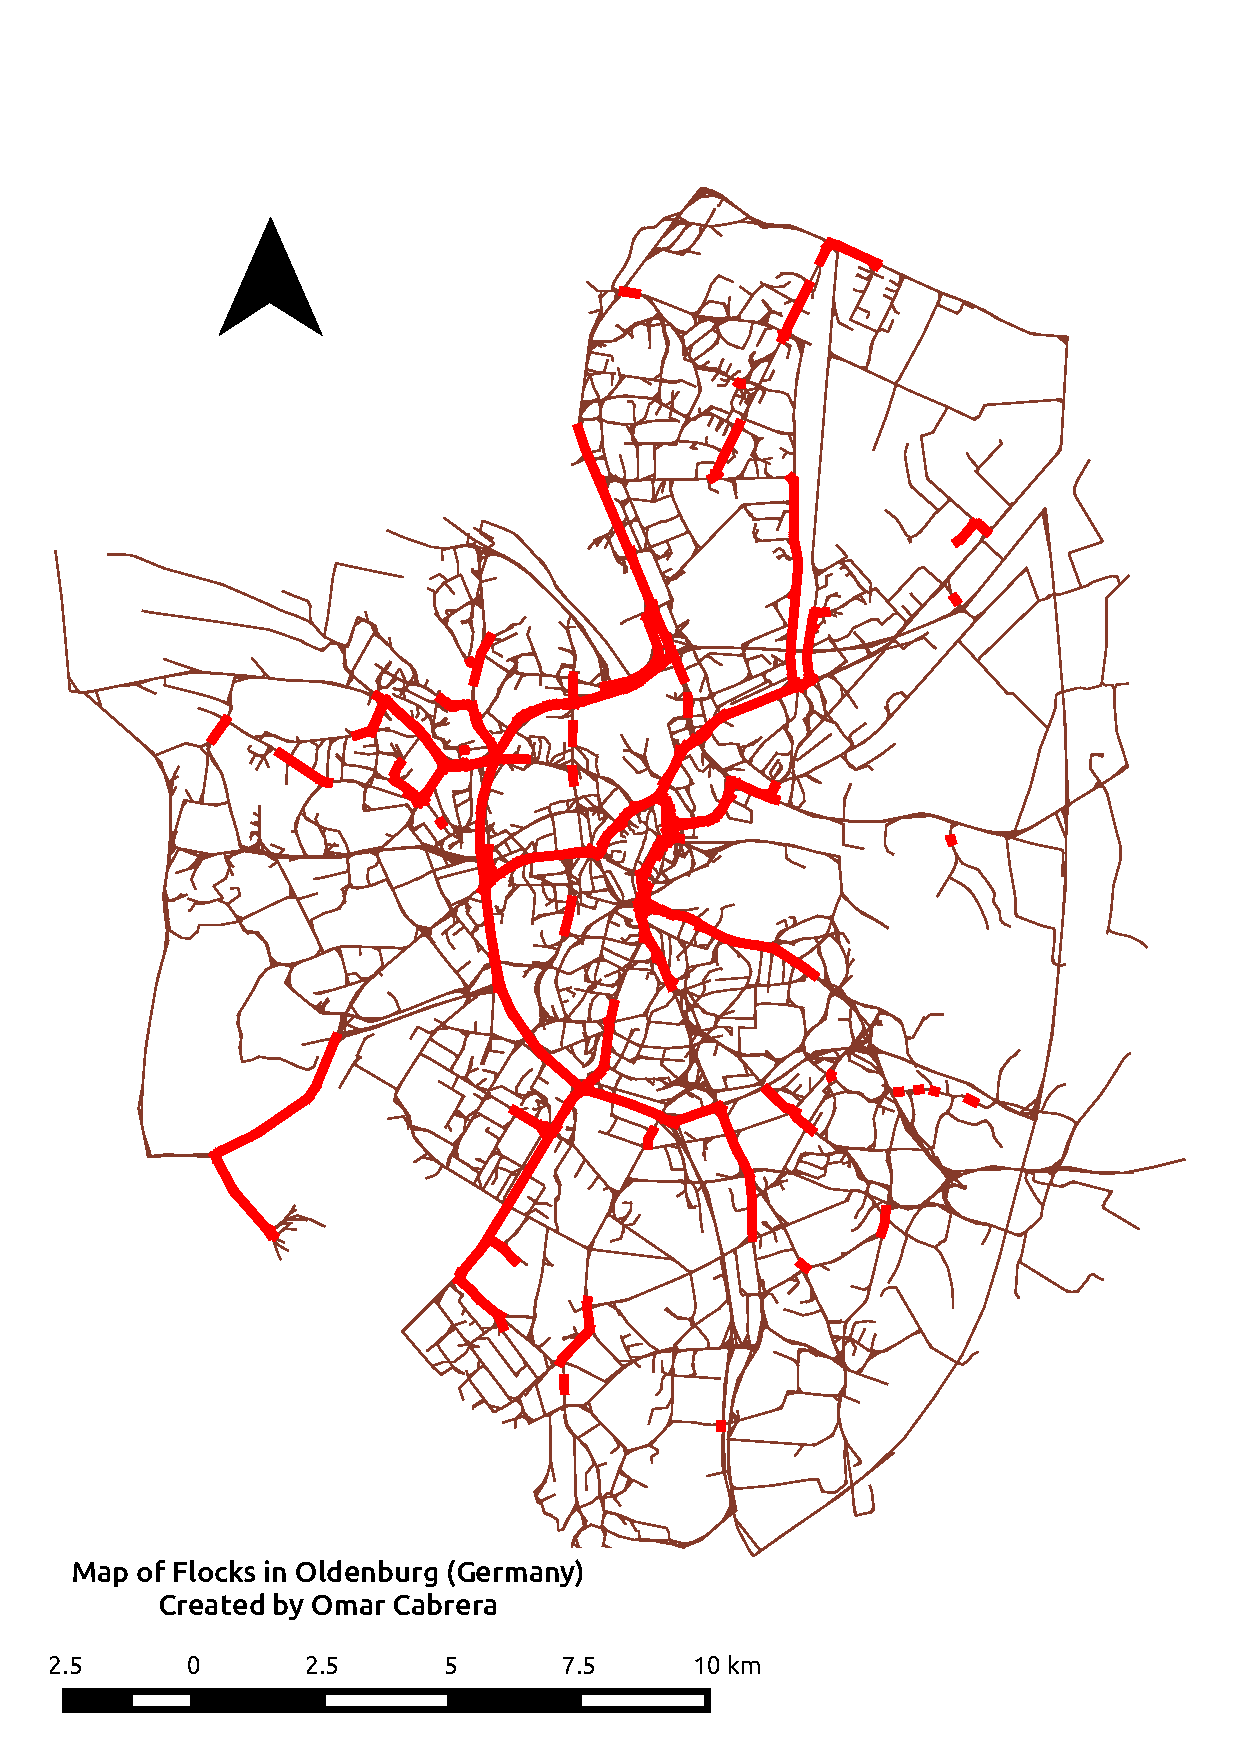
\includegraphics[scale=0.3]{pictures/bfe.pdf}}
  \subfigure[LCMFlock]{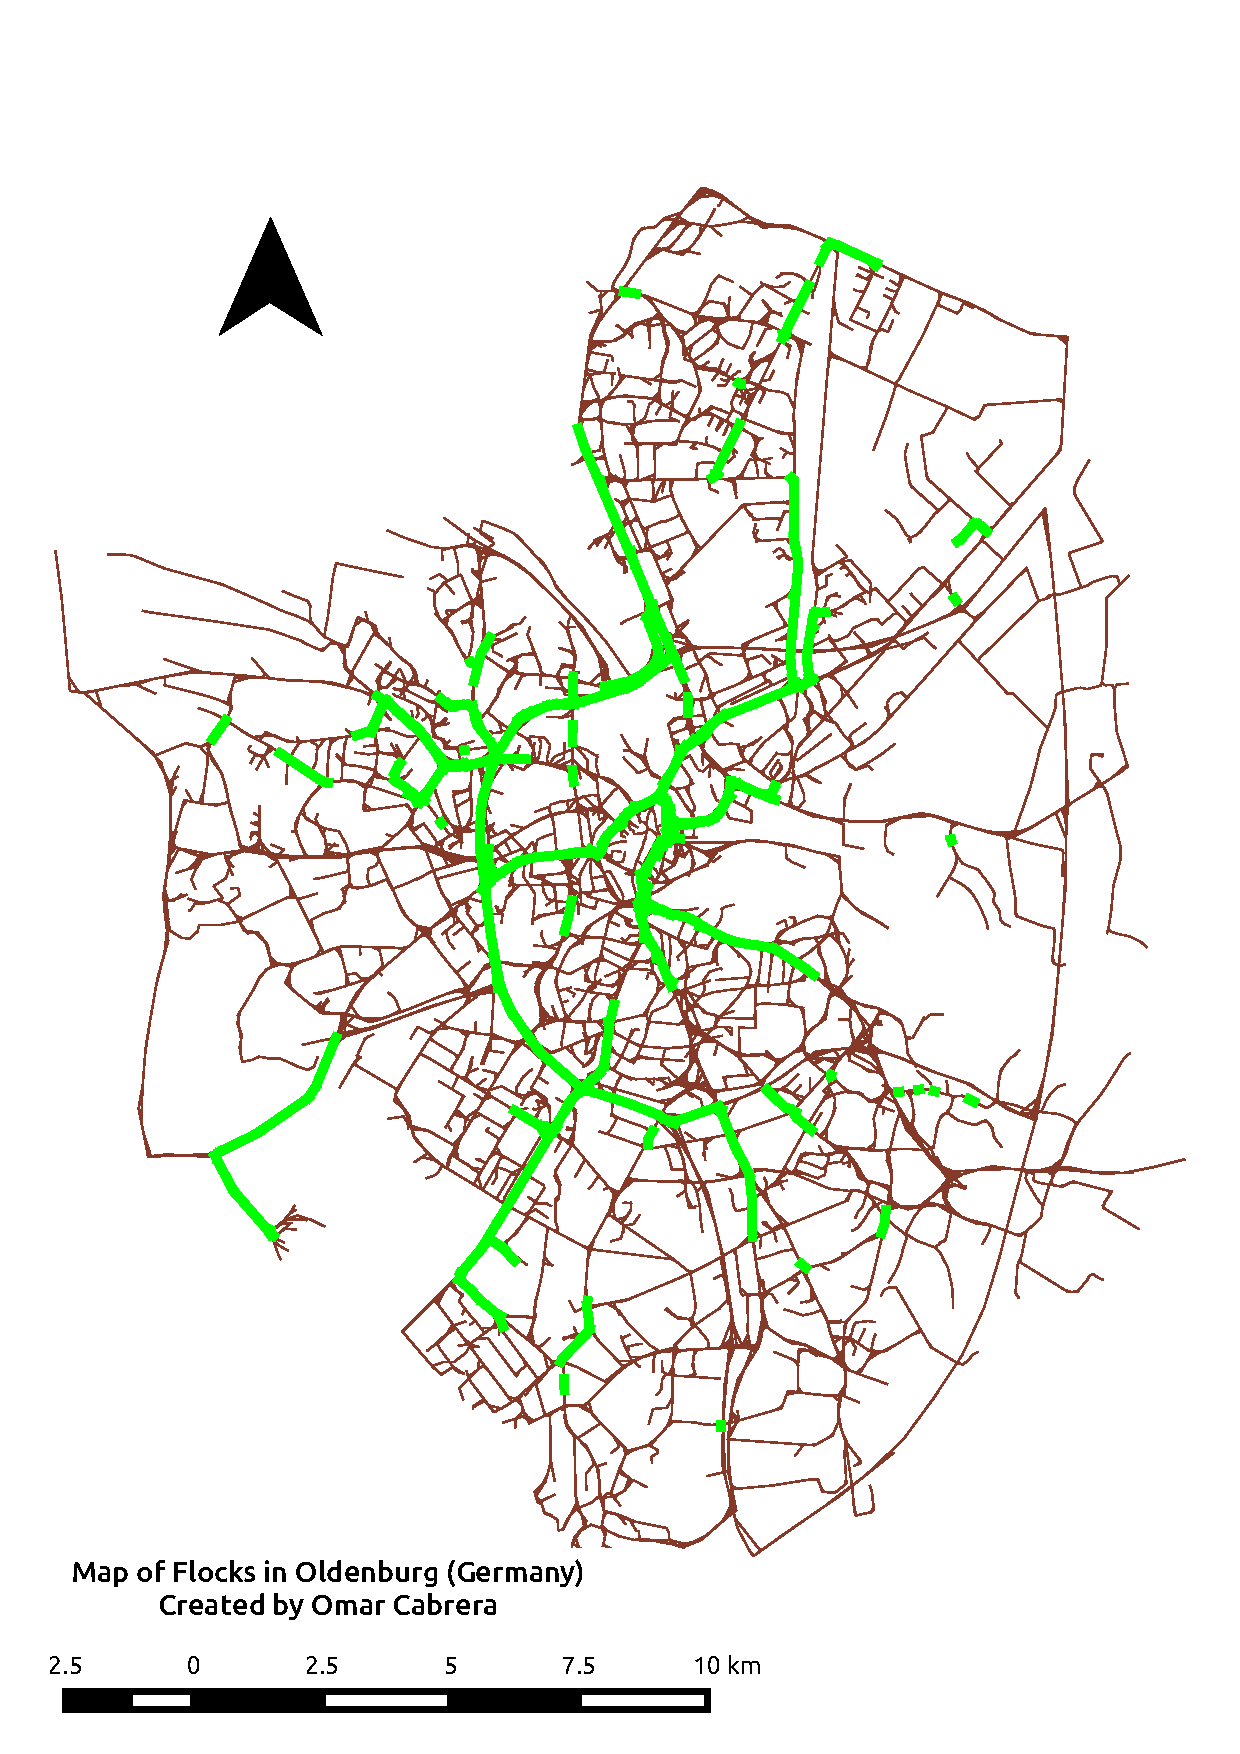
\includegraphics[scale=0.3]{pictures/lcm.pdf}}
  \subfigure[FP-FlockOnline]{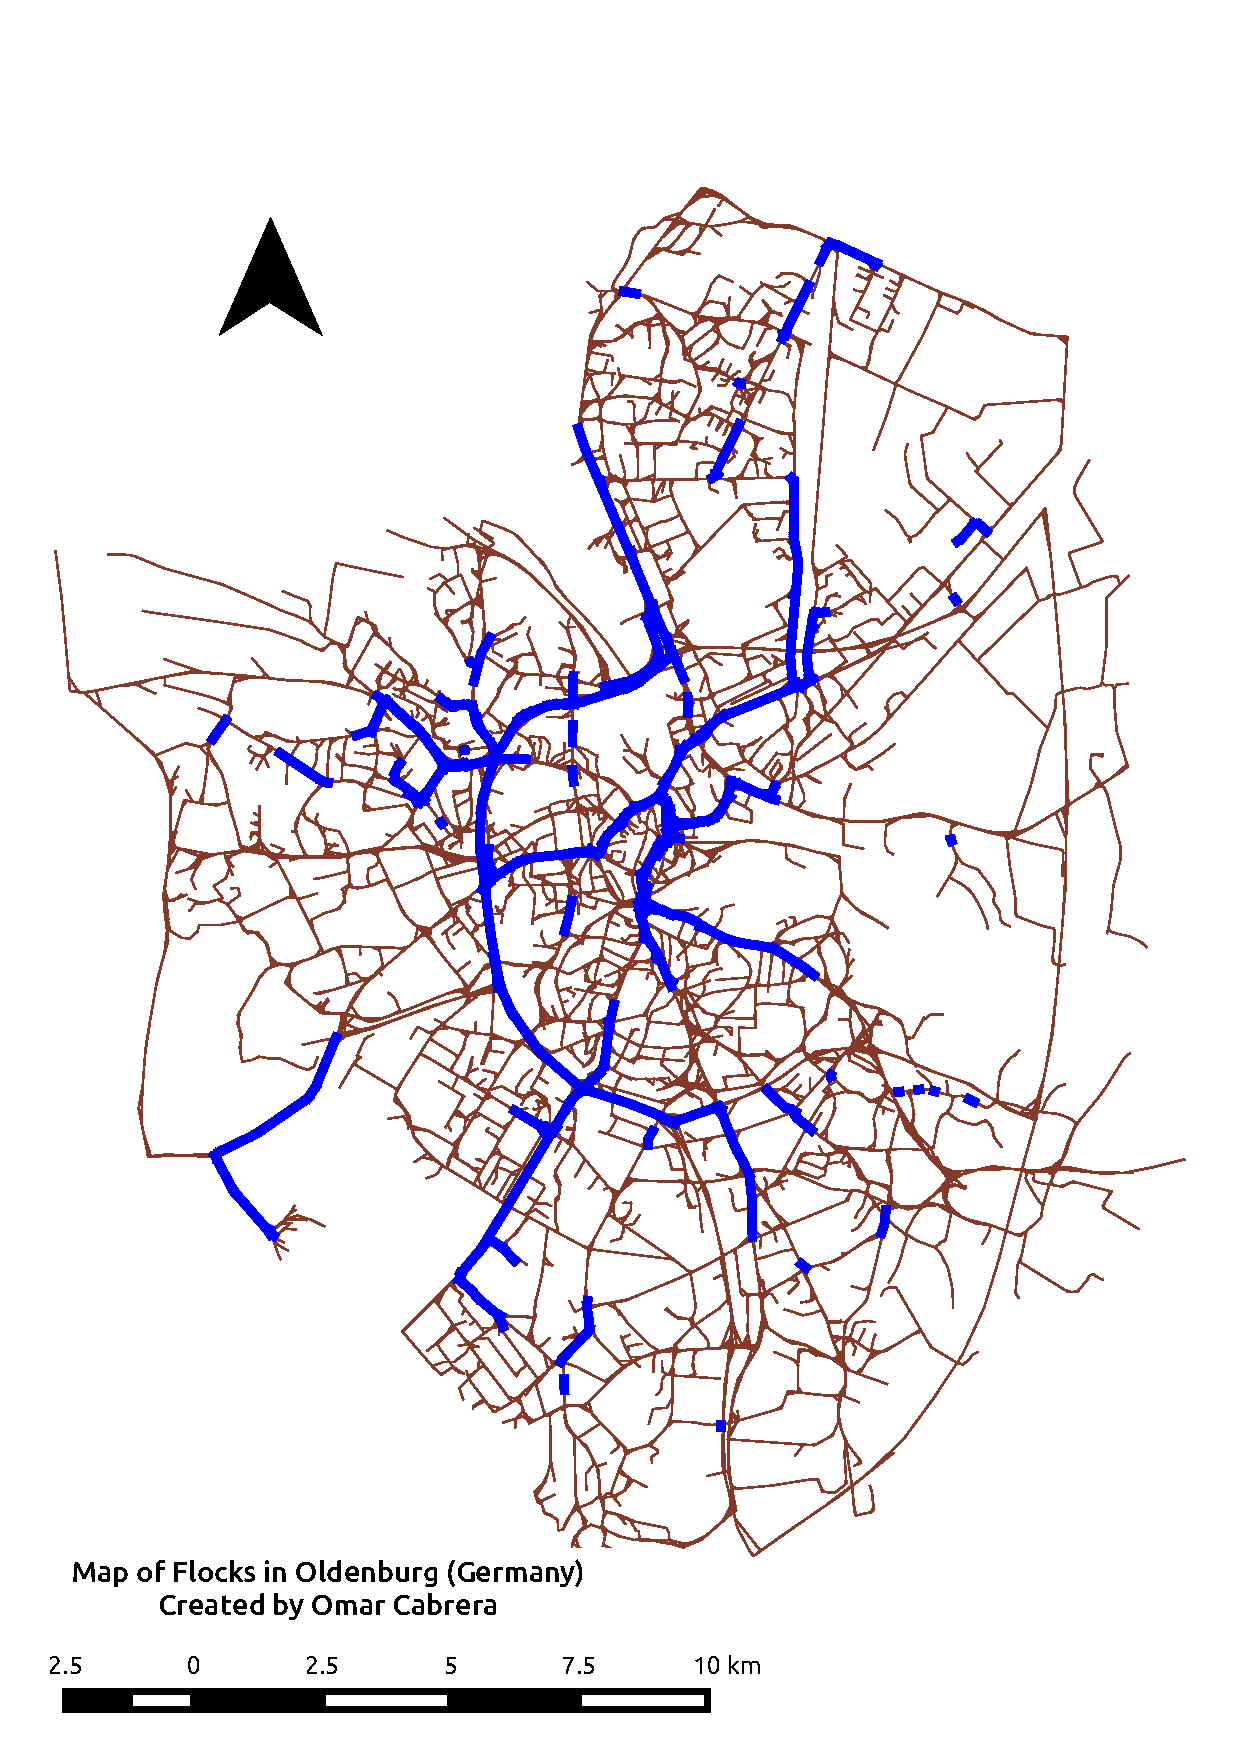
\includegraphics[scale=0.3]{pictures/fpflockOnline.pdf}}
  \subfigure[FP-FlockOffline]{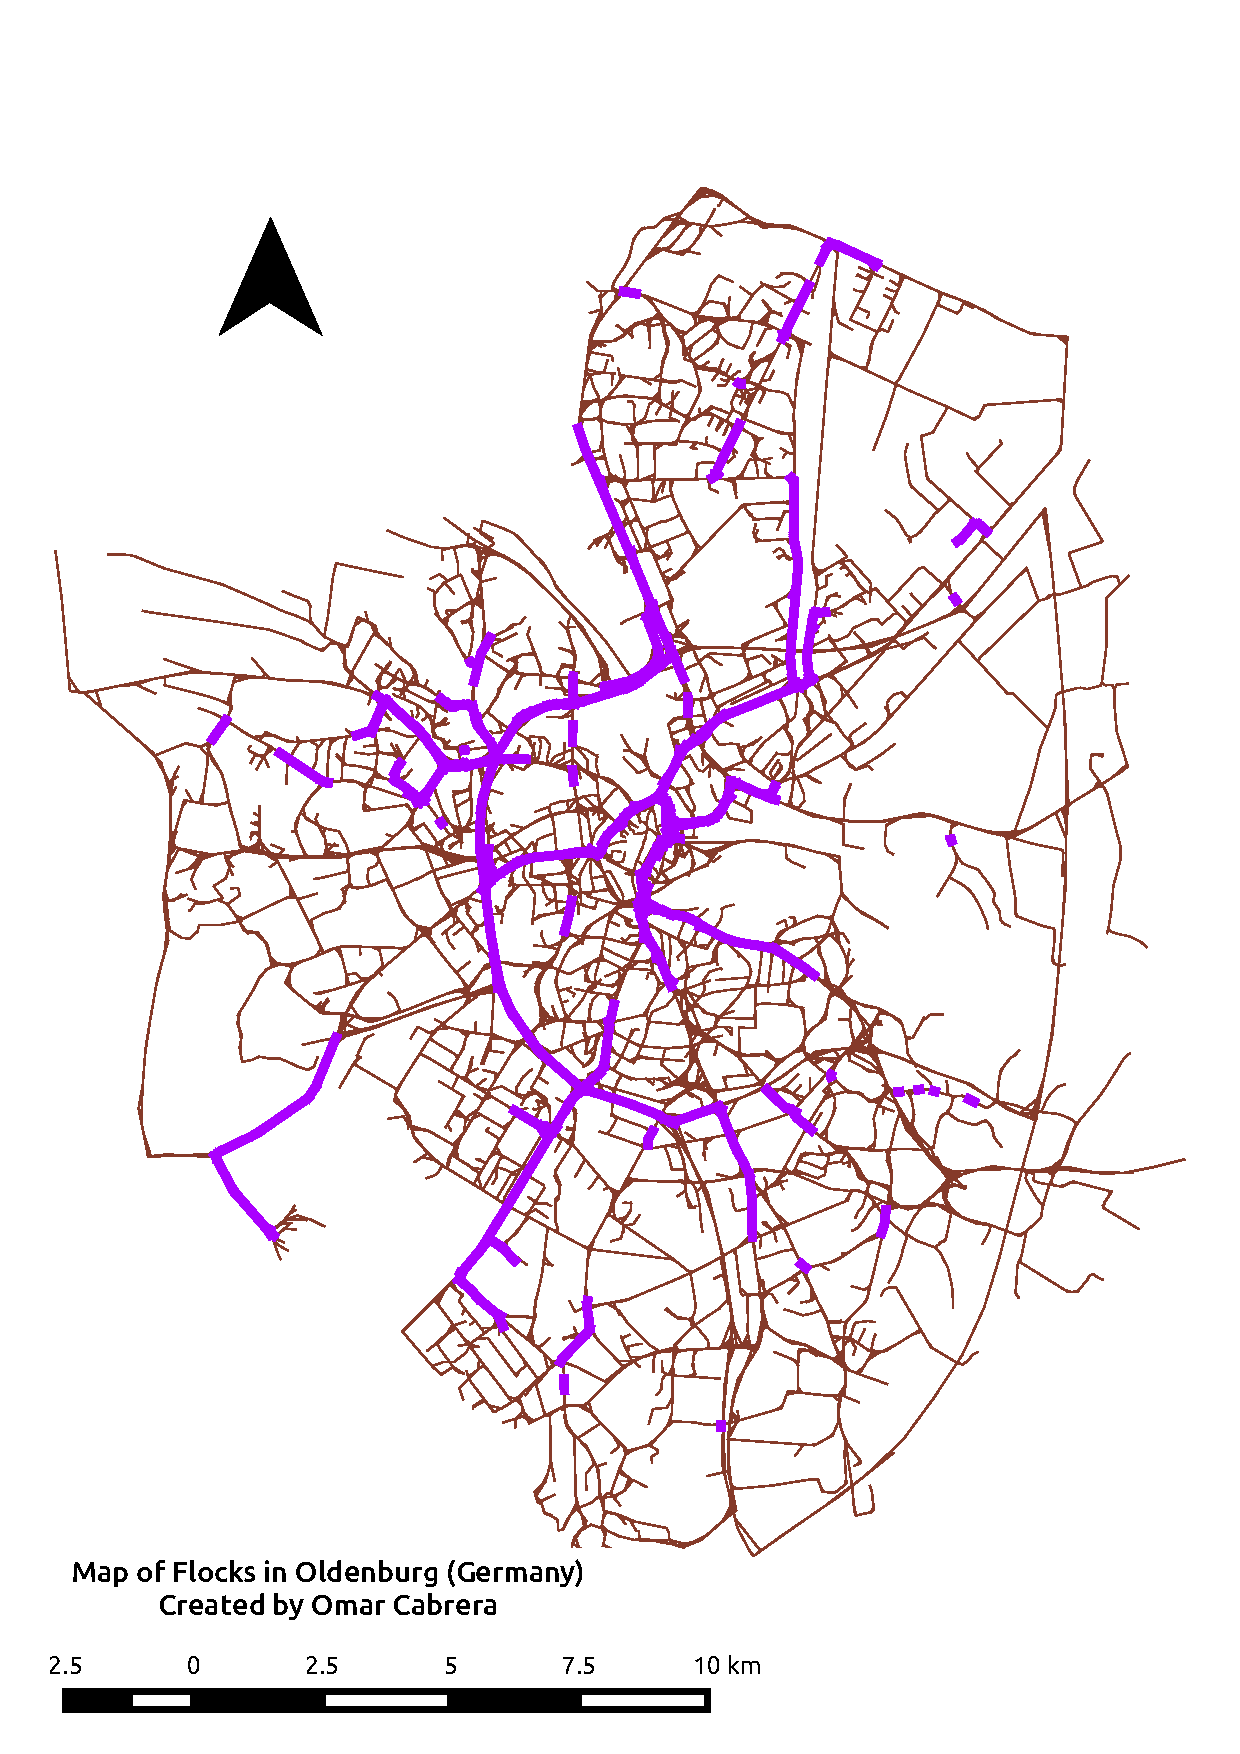
\includegraphics[scale=0.3]{pictures/fpflockOffline.pdf}}
  
  \caption{Visualización Oldenburg}
  \label{fig:validation}
\end{figure}

% \chapter{EXPERIMENTACIÓN COMPUTACIONAL}

Los resultados fueron producidos usando conjuntos de datos sintéticos y reales 
en una máquina
Dell OPTIPLEX 7010 con procesador Intel\textregistered Core\texttrademark  
i7-3770 CPU de 3.40GHz x 8,
16 GB de RAM y 1TB 7200 RPM de Disco Duro, corriendo el Sistema Operativo Debian con linux 3.2. Para 
todos los casos se usaron
los algoritmos implementados en Python, versión 3.

\section{SAN JOAQUIN}

Un grupo de conjuntos de datos sintéticos fueron creados usando un modelo para 
la generación de objetos en movimiento, como se describe en 
\cite{brinkhoff2002framework}.
Dos conjuntos de datos sintéticos fueron creados usando la red de San Joaquín 
proporcionada en el sitio web del generador \cite{Brin:2010:Online}.
El primer conjunto de datos recoge 992140 lugares simulados para 25.000 objetos 
en movimiento durante 60 instantes de tiempo. El segundo recoge 50.000 
trayectorias a partir de 2.014.346 de puntos durante 55 instantes de tiempo. La 
tabla~\ref{tab:datasets}, resume la información principal. Las 
figuras~\ref{fig:SJ25K60} y~\ref{fig:SJ50K55} muestran los tiempos de desempeño 
para estos dos casos de estudio, los parámetros adicionales fueron $\mu$=5, 
$\delta$=3 y  $\mu$=9, $\delta$=3, respectivamente.


\begin{table*}
\caption{Conjunto de datos}
\label{tab:datasets}
\centering
\begin{tabular}{c c r r c}
\toprule
\multirow{2}{*}{Dataset}& \multirow{2}{*}{Red}& \multicolumn{1}{c}{Número de}& 
Número de  & Duración promedio\\
                        &                         & trayectorias & 
\multicolumn{1}{c}{puntos} & de la trayectoria\\
\midrule
SJ25KT60  & San Joaquin & 25000 & 992140  & 40\\
SJ50KT55  & San Joaquin & 50000 & 2014346 & 37\\
TAPAS Cologne  & Cologne, Alemania & 88668 & 3403463 & 38\\
Beijing\_Original   & Beijing, China   & 21573 & 1411846& 65\\
Beijing\_Alternativo   & Beijing, China   & 18700 & 815657 & 43\\
\bottomrule
\end{tabular}\par
\bigskip
\end{table*}

\begin{figure*}
  \centering
  \subfigure[BFE, LCMFlock, FPFlock]{\label{SJ25KT60A} 
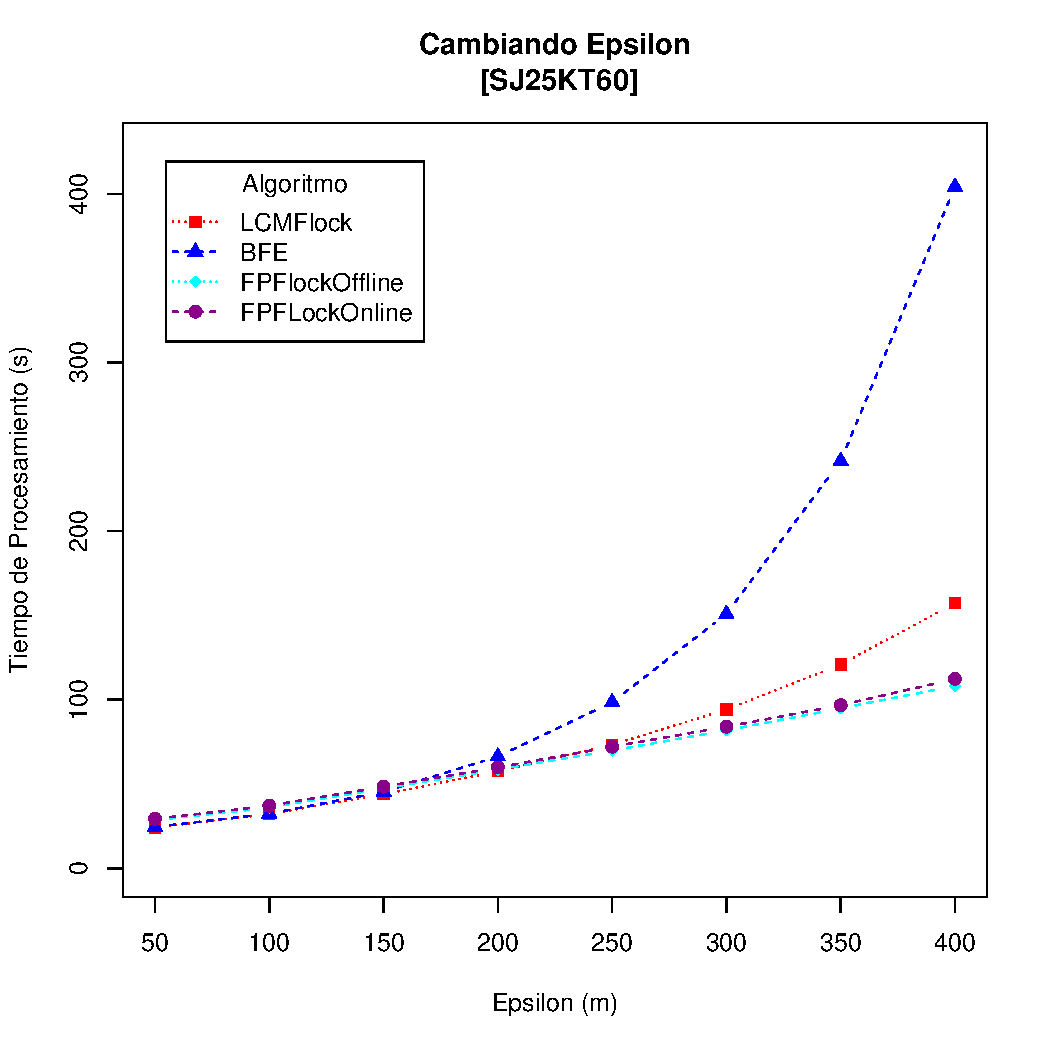
\includegraphics[scale=0.55]{pictures/SJ25KT60.pdf}}
  \subfigure[LCMFlock, 
FPFlock]{\label{SJ25KT60B}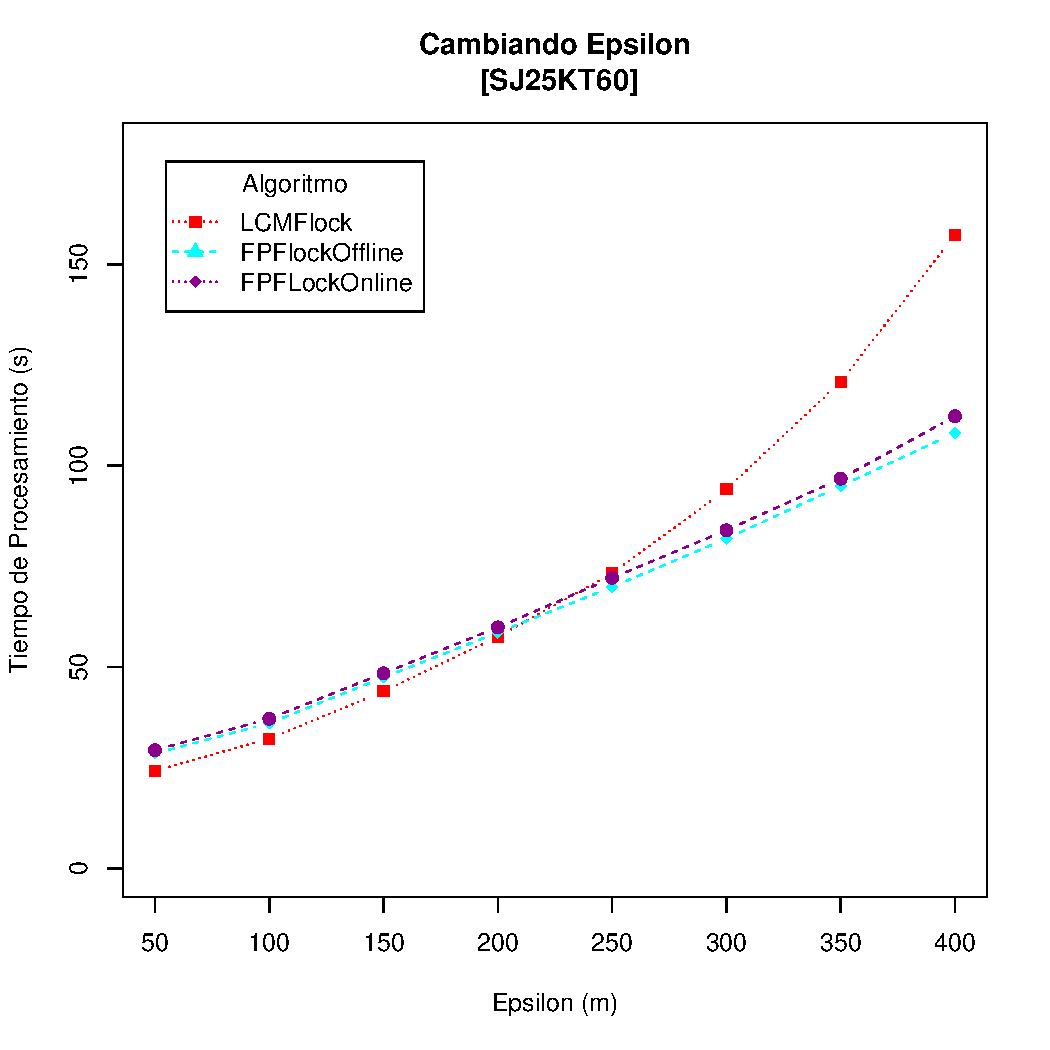
\includegraphics[scale=0.55]{pictures/SJ25KT60_B.pdf}}
  \caption{Caso de Prueba: SJ25KT60. (a) BFE, LCMFlock, FPFlock (b) LCMFlock, FPFlock}
  \label{fig:SJ25K60}
\end{figure*}

\begin{figure*}
  \centering
  \subfigure[BFE, LCMFlock, FP-Flock]{\label{SJ50K55A} 
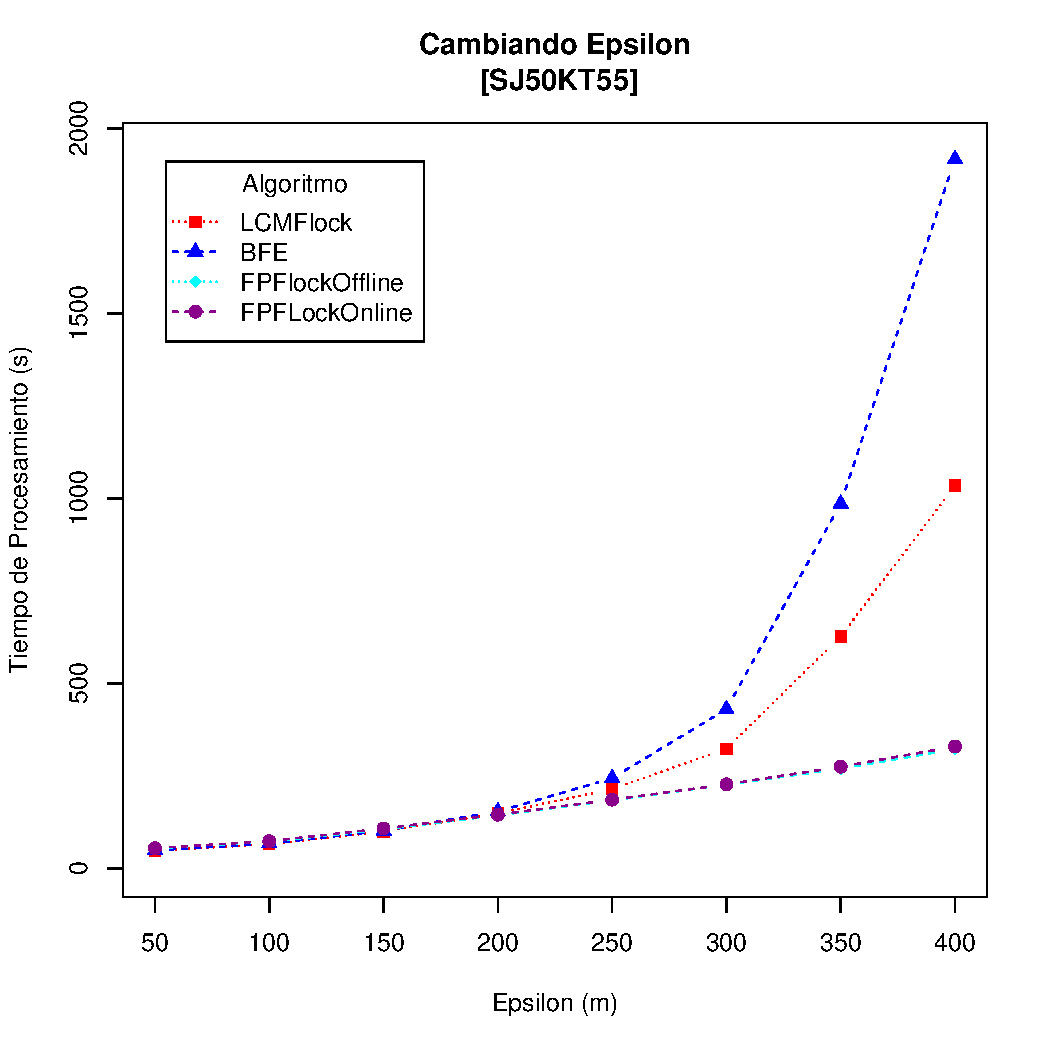
\includegraphics[scale=0.55]{pictures/SJ50KT55.pdf}}
  \subfigure[LCMFlock, FP-Flock]{\label{SJ50K55B} 
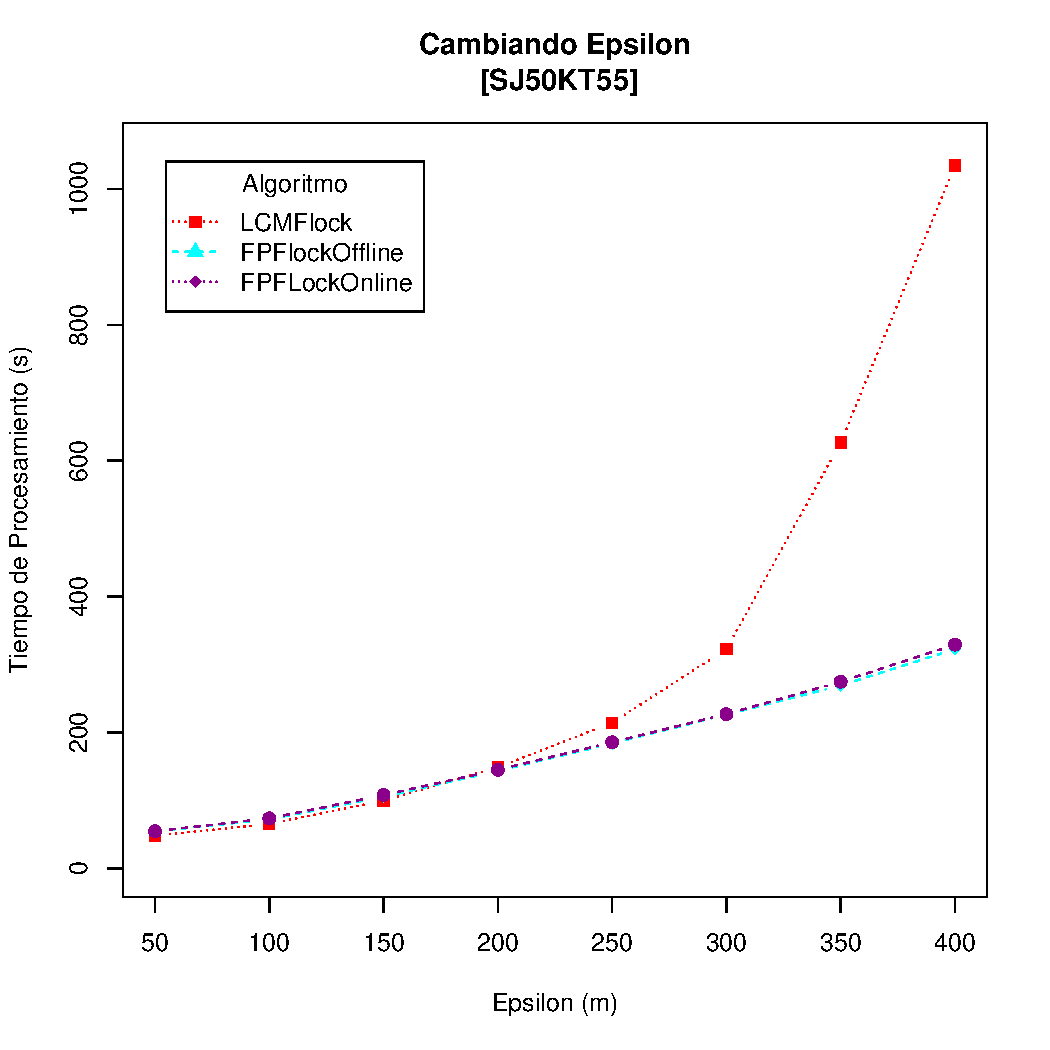
\includegraphics[scale=0.55]{pictures/SJ50KT55_B.pdf}}
  \caption{Caso de Prueba: SJ50KT55. (a) BFE, LCMFlock, FP-Flock (b) LCMFlock, FP-Flock}
  \label{fig:SJ50K55}
\end{figure*}

\section{TAPAS COLOGNE}

Este conjunto de datos sintético se preparó utilizando el escenario TAPAS 
Cologne \cite{varschen2006mikroskopische}
en SUMO \cite{krajzewicz2002sumo}, un reconocido simulador de tráfico para la 
movilidad urbana. El escenario de simulación 
TAPAS Cologne, describe el tráfico dentro de la ciudad de Colonia (Alemania) 
durante un día entero. La principal ventaja de 
este conjunto de datos es que sus trayectorias no se generan aleatoriamente. Los 
datos de la demanda original, se deriva de TAPAS, 
un sistema que calcula la tendencia de movilidad para una población con base en 
la información sobre los hábitos de viaje 
de los alemanes y en la información sobre la infraestructura de la zona en que 
viven \cite{MiD2002}. El conjunto de datos original 
es enorme por lo que sólo está disponible al público la versión de 2 horas 
\cite{TAPASCologne}. Debido a las restricciones de memoria,
se podaron las trayectorias más cortas que 20 minutos. El último conjunto de 
datos recoge 88.668 trayectorias y más 
de 3,4 millones de puntos. La tabla~\ref{tab:datasets}, describe los detalles 
sobre el conjunto de datos. Las figura~\ref{fig:Tapas} muestra los tiempos de 
desempeño para este caso de estudio. Los parámetros adicionales fueron $\mu$=10, 
$\delta$=5.

\begin{figure*}
  \centering
  \subfigure[BFE, LCMFlock, FP-Flock]{\label{tapasA} 
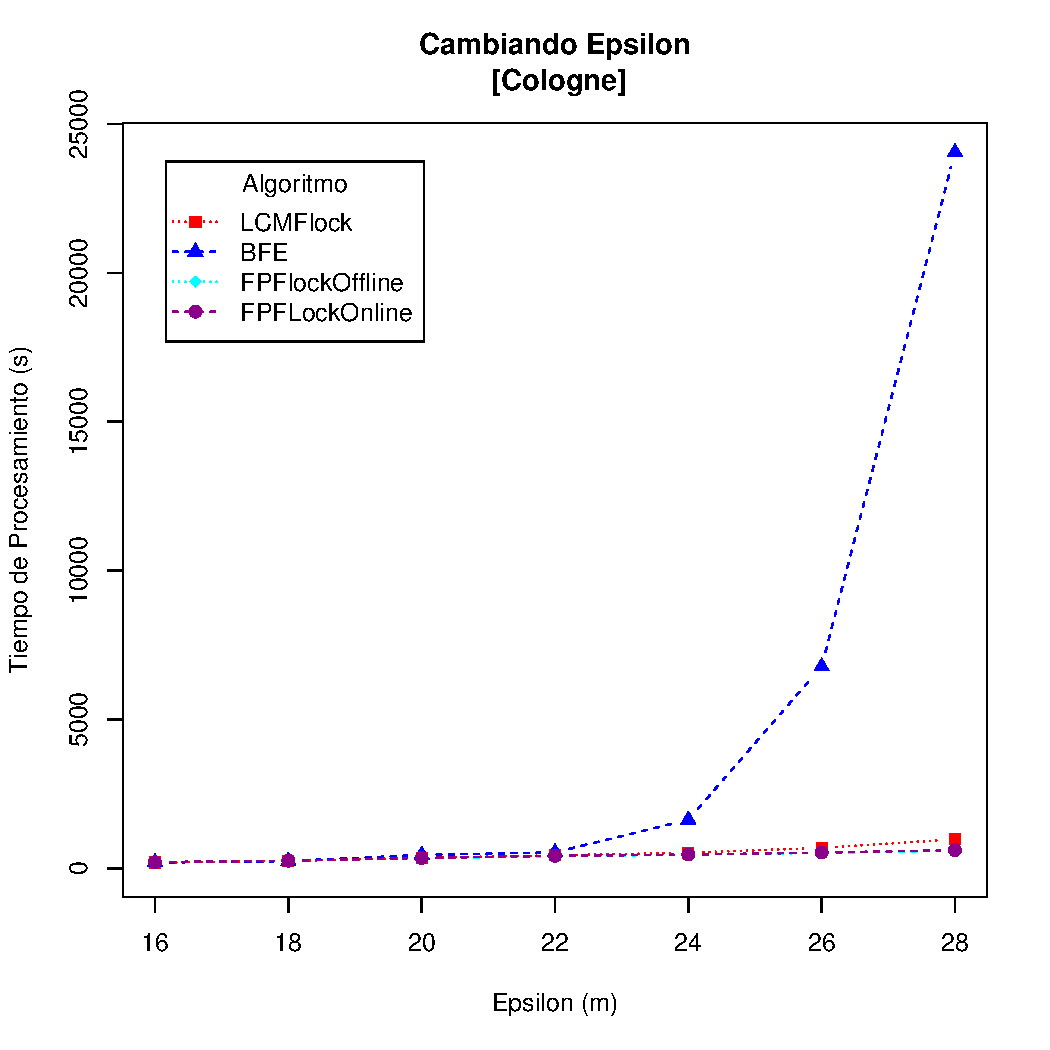
\includegraphics[scale=0.55]{pictures/Cologne.pdf}}
  \subfigure[LCMFlock, FP-Flock]{\label{tapasB} 
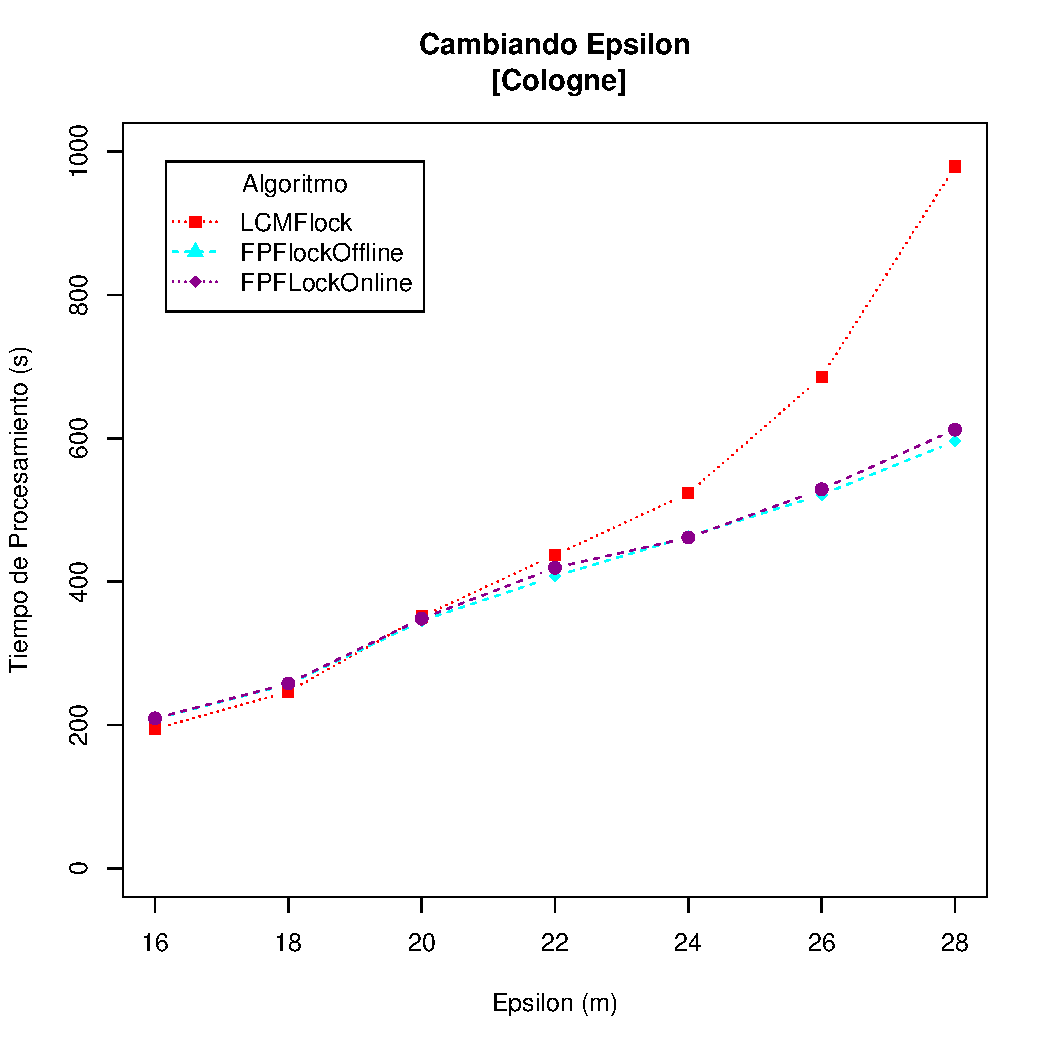
\includegraphics[scale=0.55]{pictures/Cologne_B.pdf}}  
  \caption{Caso de Prueba: Tapas Cologne. (a) BFE, LCMFlock, FP-Flock (b) LCMFlock, FP-Flock}
  \label{fig:Tapas}
\end{figure*}

\section{MOVIMIENTO DE PEATONES EN BEIJING}

Este conjunto de datos reales recopila información de movimiento de un grupo de 
personas en toda
el área metropolitana de Beijing, China\cite{GeoLife}. El conjunto de datos se 
recogió durante el proyecto Geolife por 165 usuarios anónimos en un período de 
dos años entre abril de 2007 y agosto de 2009. Las ubicaciones fueron grabadas 
por diferentes dispositivos GPS o teléfonos inteligentes y la mayoría de ellos 
presentan una frecuencia de muestreo alta. 
La región alrededor del quinto anillo vial en el área metropolitana de Beijing 
mostró la 
mayor concentración de trayectorias. Esto fue usado para generar un conjunto de 
datos de muestra. Cada trayectoria 
fue interpolada por minuto (un punto por minuto) y saltos de 20 minutos o más 
sin señal se utilizaron para marcar una nueva trayectoria. Por último, el 
conjunto de datos recoge más 
de 1,4 millones de puntos y 21.573 trayectorias. Sin embargo, como este conjunto 
de datos tuvo poca cantidad de
entidades en movimiento (165 usuarios) en una ventana de tiempo de más de 2 
años, no existieron muchas trayectorias ocurriendo al mismo tiempo. Para probar
la escalabilidad de los algoritmos, se decidió crear un conjunto de datos alternativo basado en las 
trayectorias reales, pero forzando para que todas ellas comiencen al mismo 
tiempo. Una 
vez más, por las limitaciones de memoria, las trayectorias más cortas que 10 
minutos y más largas que 3 horas se podaron. El conjunto de datos alternativo 
almacenó 815.657 
ubicaciones y 18.700 trayectorias. La tabla~\ref{tab:datasets} resume los 
detalles para ambos conjuntos de datos. Las figuras~\ref{fig:BeijingOr} 
y~\ref{fig:BeijingAl} muestran los tiempos de desempeño para estos dos casos de 
estudio, los parámetros adicionales fueron $\mu$=3, $\delta$=3 y  $\mu$=5, 
$\delta$=5 respectivamente.


\begin{figure}
  \centering
  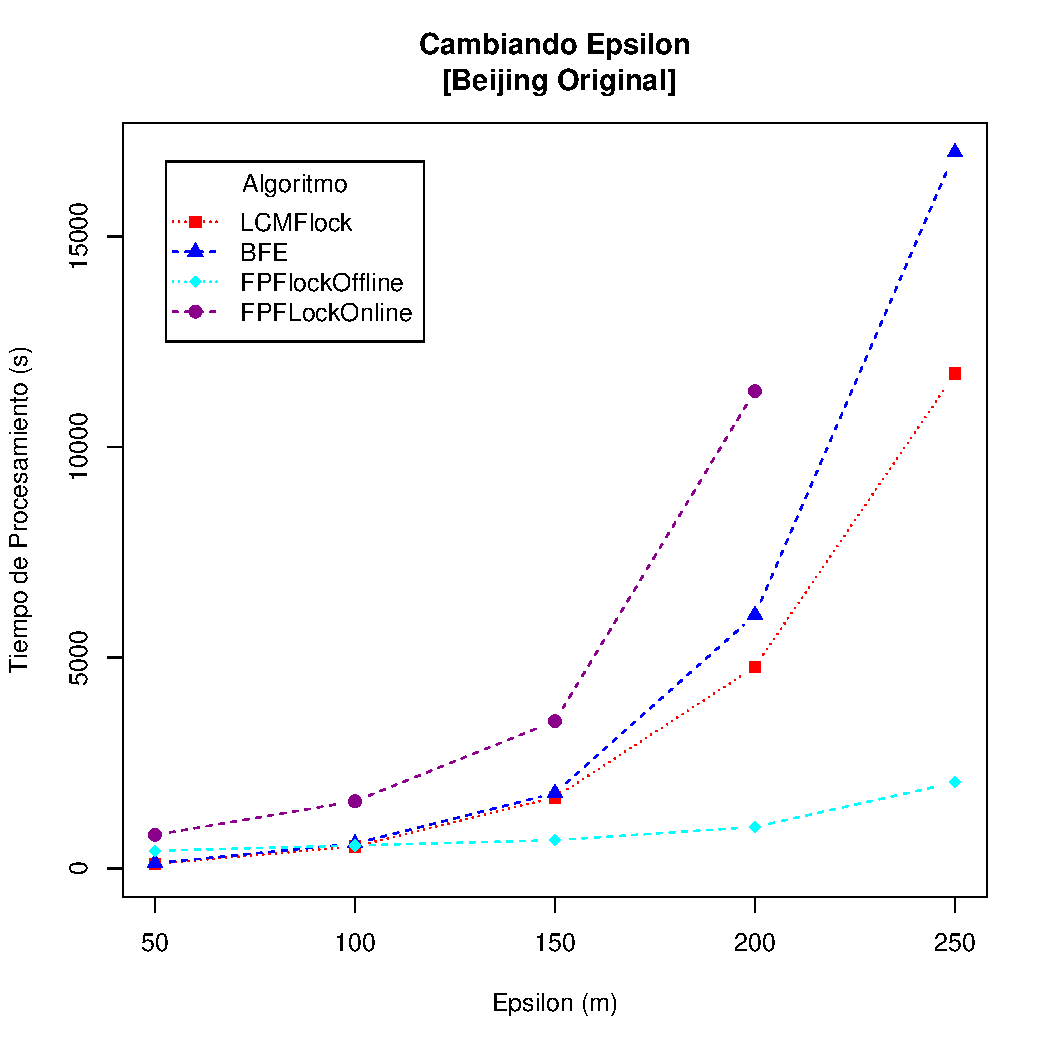
\includegraphics[scale=0.55]{pictures/Beijing_Original.pdf}
  \caption{Caso de Prueba: Beijing Original}
  \label{fig:BeijingOr}
\end{figure}

\begin{figure*}
  \centering
  \subfigure[BFE, LCMFlock, FP-Flock]{\label{b1} 
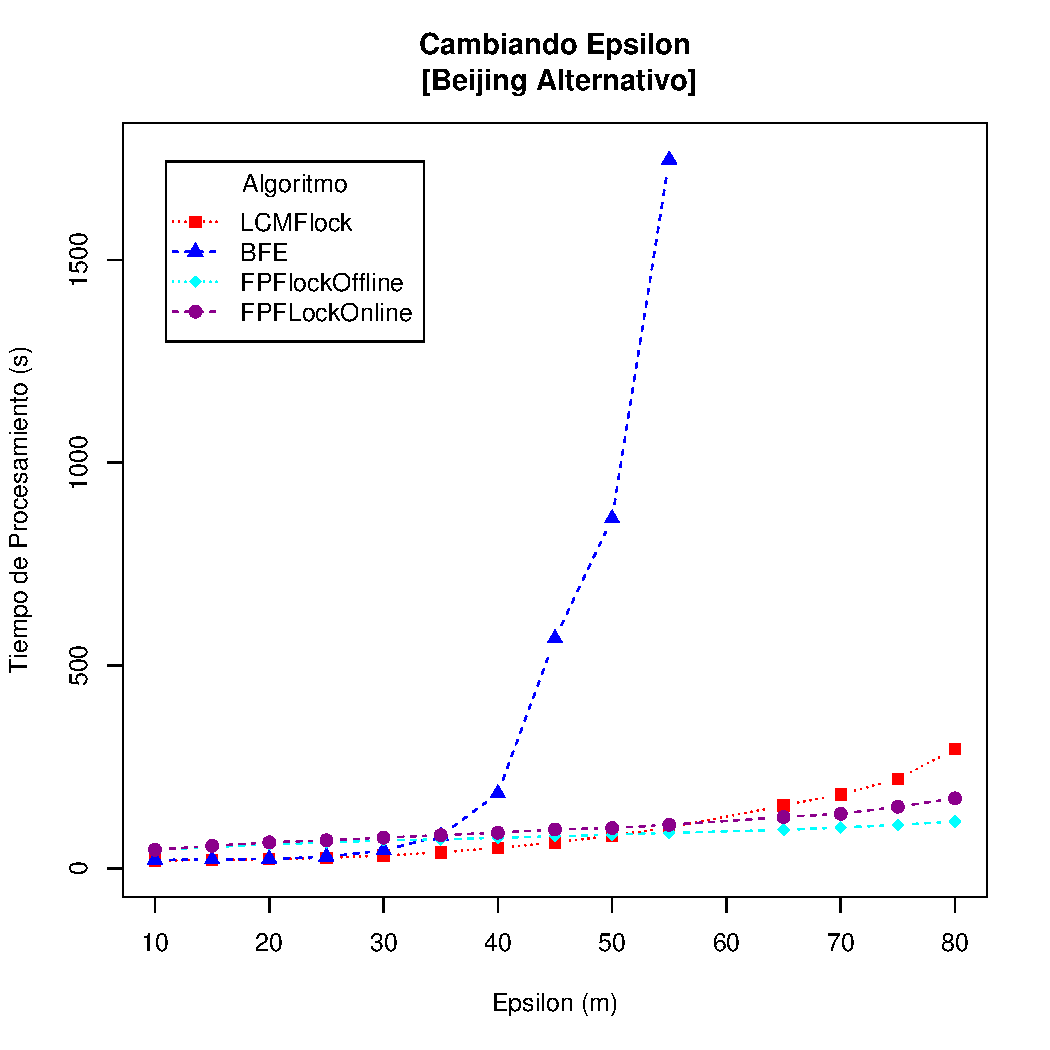
\includegraphics[scale=0.55]{pictures/Beijing_Alternativo.pdf}}
  \subfigure[LCMFlock, FP-Flock]{\label{b2} 
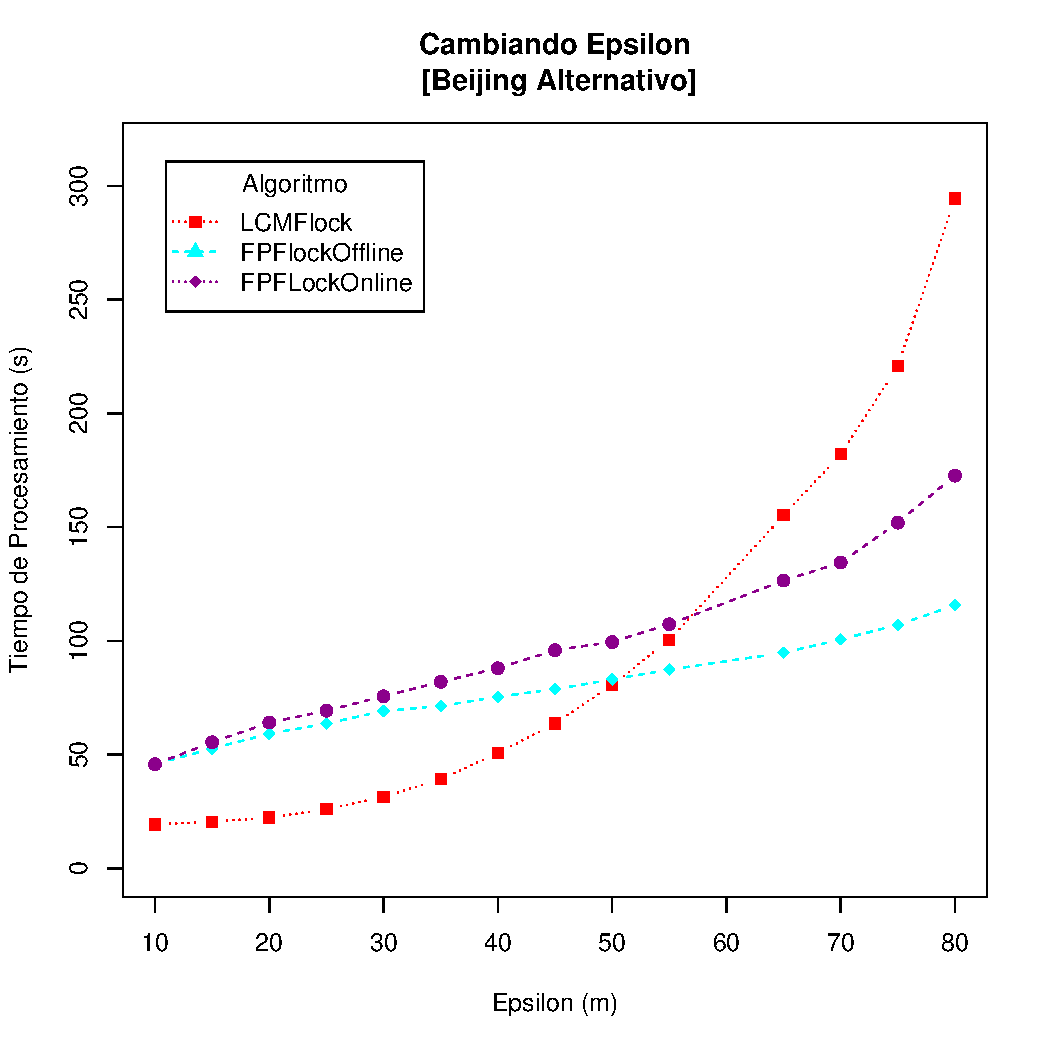
\includegraphics[scale=0.55]{pictures/Beijing_Alternativo_B.pdf}}
  \caption{Caso de Prueba: Beijing Alternativo. (a) BFE, LCMFlock, FP-Flock (b) LCMFlock, FP-Flock}
  \label{fig:BeijingAl}
\end{figure*}


\section{REPORTE DE FLOCKS}

Tanto para BFE, LCMFlock, FP-FlockOnline y FP-FlockOffline el reporte de flocks se hace en una base 
de datos, 
con un identificador, tiempo de inicio, tiempo de fin y todos los puntos 
contenidos en dicho flock. En la tabla~\ref{tab:flocks}, se muestra el número 
total de flocks reportados con un $\varepsilon$ en particular.

\begin{table}
\caption{Número de Flocks}
\label{tab:flocks}
\centering
\scalebox{0.8}{
\begin{tabular}{c c r r r r c}
\toprule
\multirow{2}{*}{Dataset}&  $\varepsilon$ & \multicolumn{1}{c}{Número de Flocks}& Número de Flocks & 
Número de Flocks & Número de Flocks \\
                        &                         &\multicolumn{1}{c}{BFE} & 
\multicolumn{1}{c}{LCMFlock} & \multicolumn{1}{c}{FP-FlockOnline} & 
\multicolumn{1}{c}{FP-FlockOffline}  \\
                        
\midrule
SJ25KT60  & 300 & 35805 & 5466 & 26877 & 5466\\
SJ50KT55  & 300 & 45201 & 6396 & 23638 & 6396\\
TAPAS Cologne  & 28  & 9415451 & 31509 & 145217 & 31509\\
Beijing\_Original   & 250   & 16628029 & 4373139 & - & 4373139\\
Beijing\_Alternativo   & 50   & 6110427 & 19233 & 63566 & 19233\\
\bottomrule
\end{tabular}}\par
\bigskip
\end{table}

% \chapter{ CONCLUSIONES Y TRABAJOS FUTUROS}

Con la culminación de esta tesis se logra  descubrir relaciones conceptuales entre los trabajos de grado de la Universidad de Nariño (Colombia) utilizando técnicas de minería de texto y facilitar la recuperación de trabajos de grado relacionados con temáticas de la búsquedas identificando similitudes y diferencias entre ellos.

Con la construcción, limpieza y transformación del repositorio de documentos de trabajos de grado de la universidad de Nariño; se logró estructurar este repositorio usando diferentes técnicas de minería de texto y se seleccionó la más adecuada que de acuerdo a los resultados fue Doc2vec.

Estructurar  el corpus de trabajos permito utilizar el algoritmo k-means, para encontrar relaciones categoriales y diferenciar los dominios de conocimiento del repositorio, los resultados mostraron que el número óptimo de categorías o grupos de conocimiento es 32.

Los modelos  Ner y  Word2vec permitieron interpretar el conocimiento relacionado a cada una de las categorías encontradas, estos 2 modelos fueron implementados en el algoritmo \ref{alg:maskanita2} el cual visualiza relaciones conceptuales temáticas  entre los documentos del repositorio. 

Las tareas de clasificación si bien sufren de sobre ajuste obtuvieron un buen desempeño, el modelo Xgboost alcanzó una medida de accuracy en el conjunto de testeo del 90\%, el cual resultó superior a los demás clasificadores, este modelo permite clasificar nuevos documentos que ingresen al repositorio y se implementó en el algoritmo \ref{alg:maskanita1};  para clasificar las temáticas de búsqueda en las categorías o grupos encontrados y con esto poder recuperar documentos similares a estas. 

Como trabajo a futuro se recomienda implementar los modelos y algoritmos realizados en esta tesis, en el domino de trabajos de investigación de la vicerrectoría de investigación de la universidad de Nariño.  




\bibliography{bibliography}
\bibliographystyle{IEEEtran}
\addcontentsline{toc}{chapter}{REFERENCIAS}

%\chapter*{ ANEXOS}
%\addcontentsline{toc}{chapter}{ANEXOS}

%\begin{itemize}
 %\item Poster presentado en el Congreso Andino de Computación, Informática y 
%Educación (CACIED).
 %\item Artículo publicado en la Conferencia Latinoamericana en Informática (CLEI 2014).
 %\item Artículo que esta en etapa de evaluación en revista indexada ``Polibits''.
 
\end{itemize}

\end{document}

